%   Filename    : chapter_4.tex 
\chapter{Results}
%\This chapter presents the results or the system of your SP. Include screenshots, tables, or graphs and provide the discussion of results.
This chapter presents the results of the study, specifically the HanApp application suite's various interfaces and screens, features, and backend framework implementation. As such, the figures shown herein are screenshots of HanApp's release build interfaces as well as the backend framework, particularly Firebase.

\section{PNP Admin Interface}
The PNP Admin interface focuses on the managing and administrative side of the applcation suite, providing the necessary access, features, and screens to manage all missing persons reports sent by users through HanApp's main user application interface.

\subsection{PNP Account Creation and Login Screen}

Figure \ref{fig:PNP1} Login page of the PNP-side app will authenticate the user to enforce access in the reports management system of the missing persons. Input fields are provided for username and password for PNP’s credentials. When the PNP Admin user is having troubles with regards to authentication or registration, they would need to contact the developers directly, either to get an admin account for their respective PNP outpost, or to reset the password of their corresponding admin accounts. 

\subsubsection{PNP Account Locations}

For the proof of concept, four hard-coded PNP accounts, namely; PNP Miagao, PNP San Joaqin, PNP Jaro, and the National PNP were created by the developers directly through Firebase console's Authentication page. These accounts have the corresponding location (their "location data") of the PNP outposts in their locality (i.e. PNP San Joaqin account has the location of San Joaqin PNP outpost). 

The PNP location data are utilized to filter out where the reports, based on their MP's last seen location, should be filtering to. However, it's important to note that the National PNP account will receive all reports regardless of distance, this is in order to cater to the reports filed outside of the vicinity of the Miagao, San Joaqin, and  Jaro PNP accounts.

\begin{figure}[!h]
    \centering
    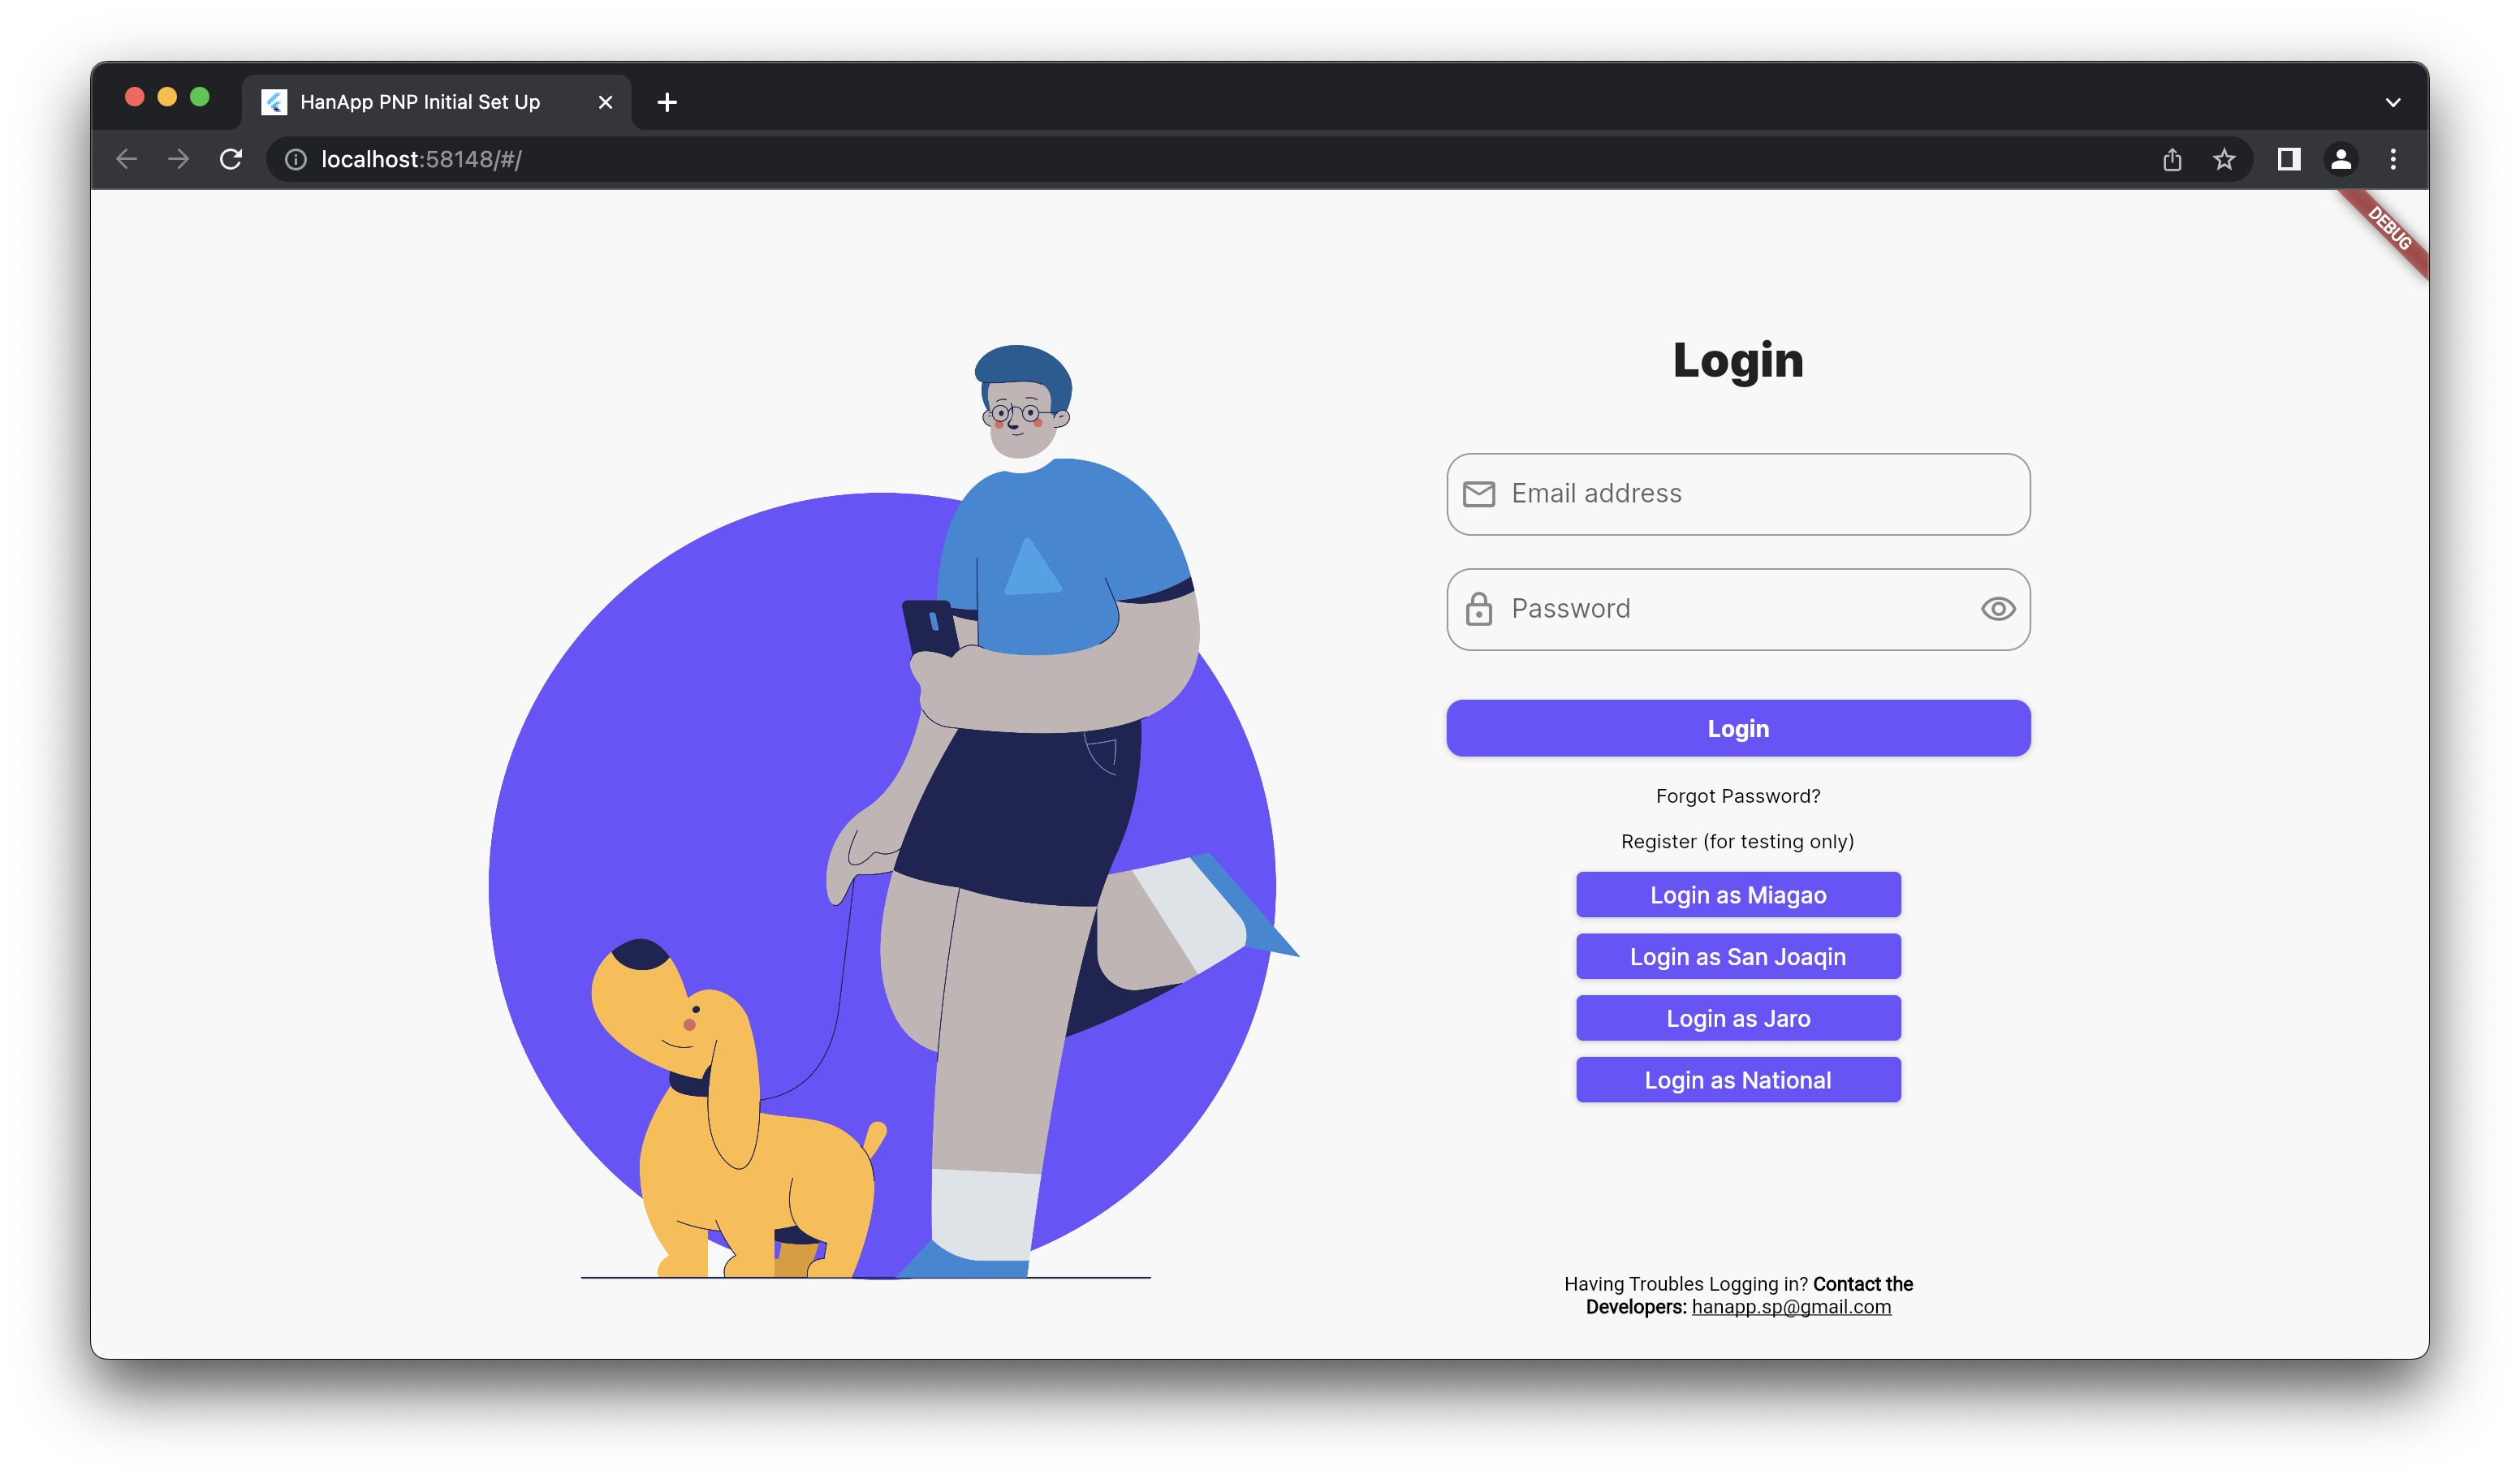
\includegraphics[scale=0.25]{figures/Chapter4/PNP/Login.png}
    \caption{PNP Admin Login Page}
    \label{fig:PNP1}
\end{figure}

\begin{figure}[!h]
    \centering
    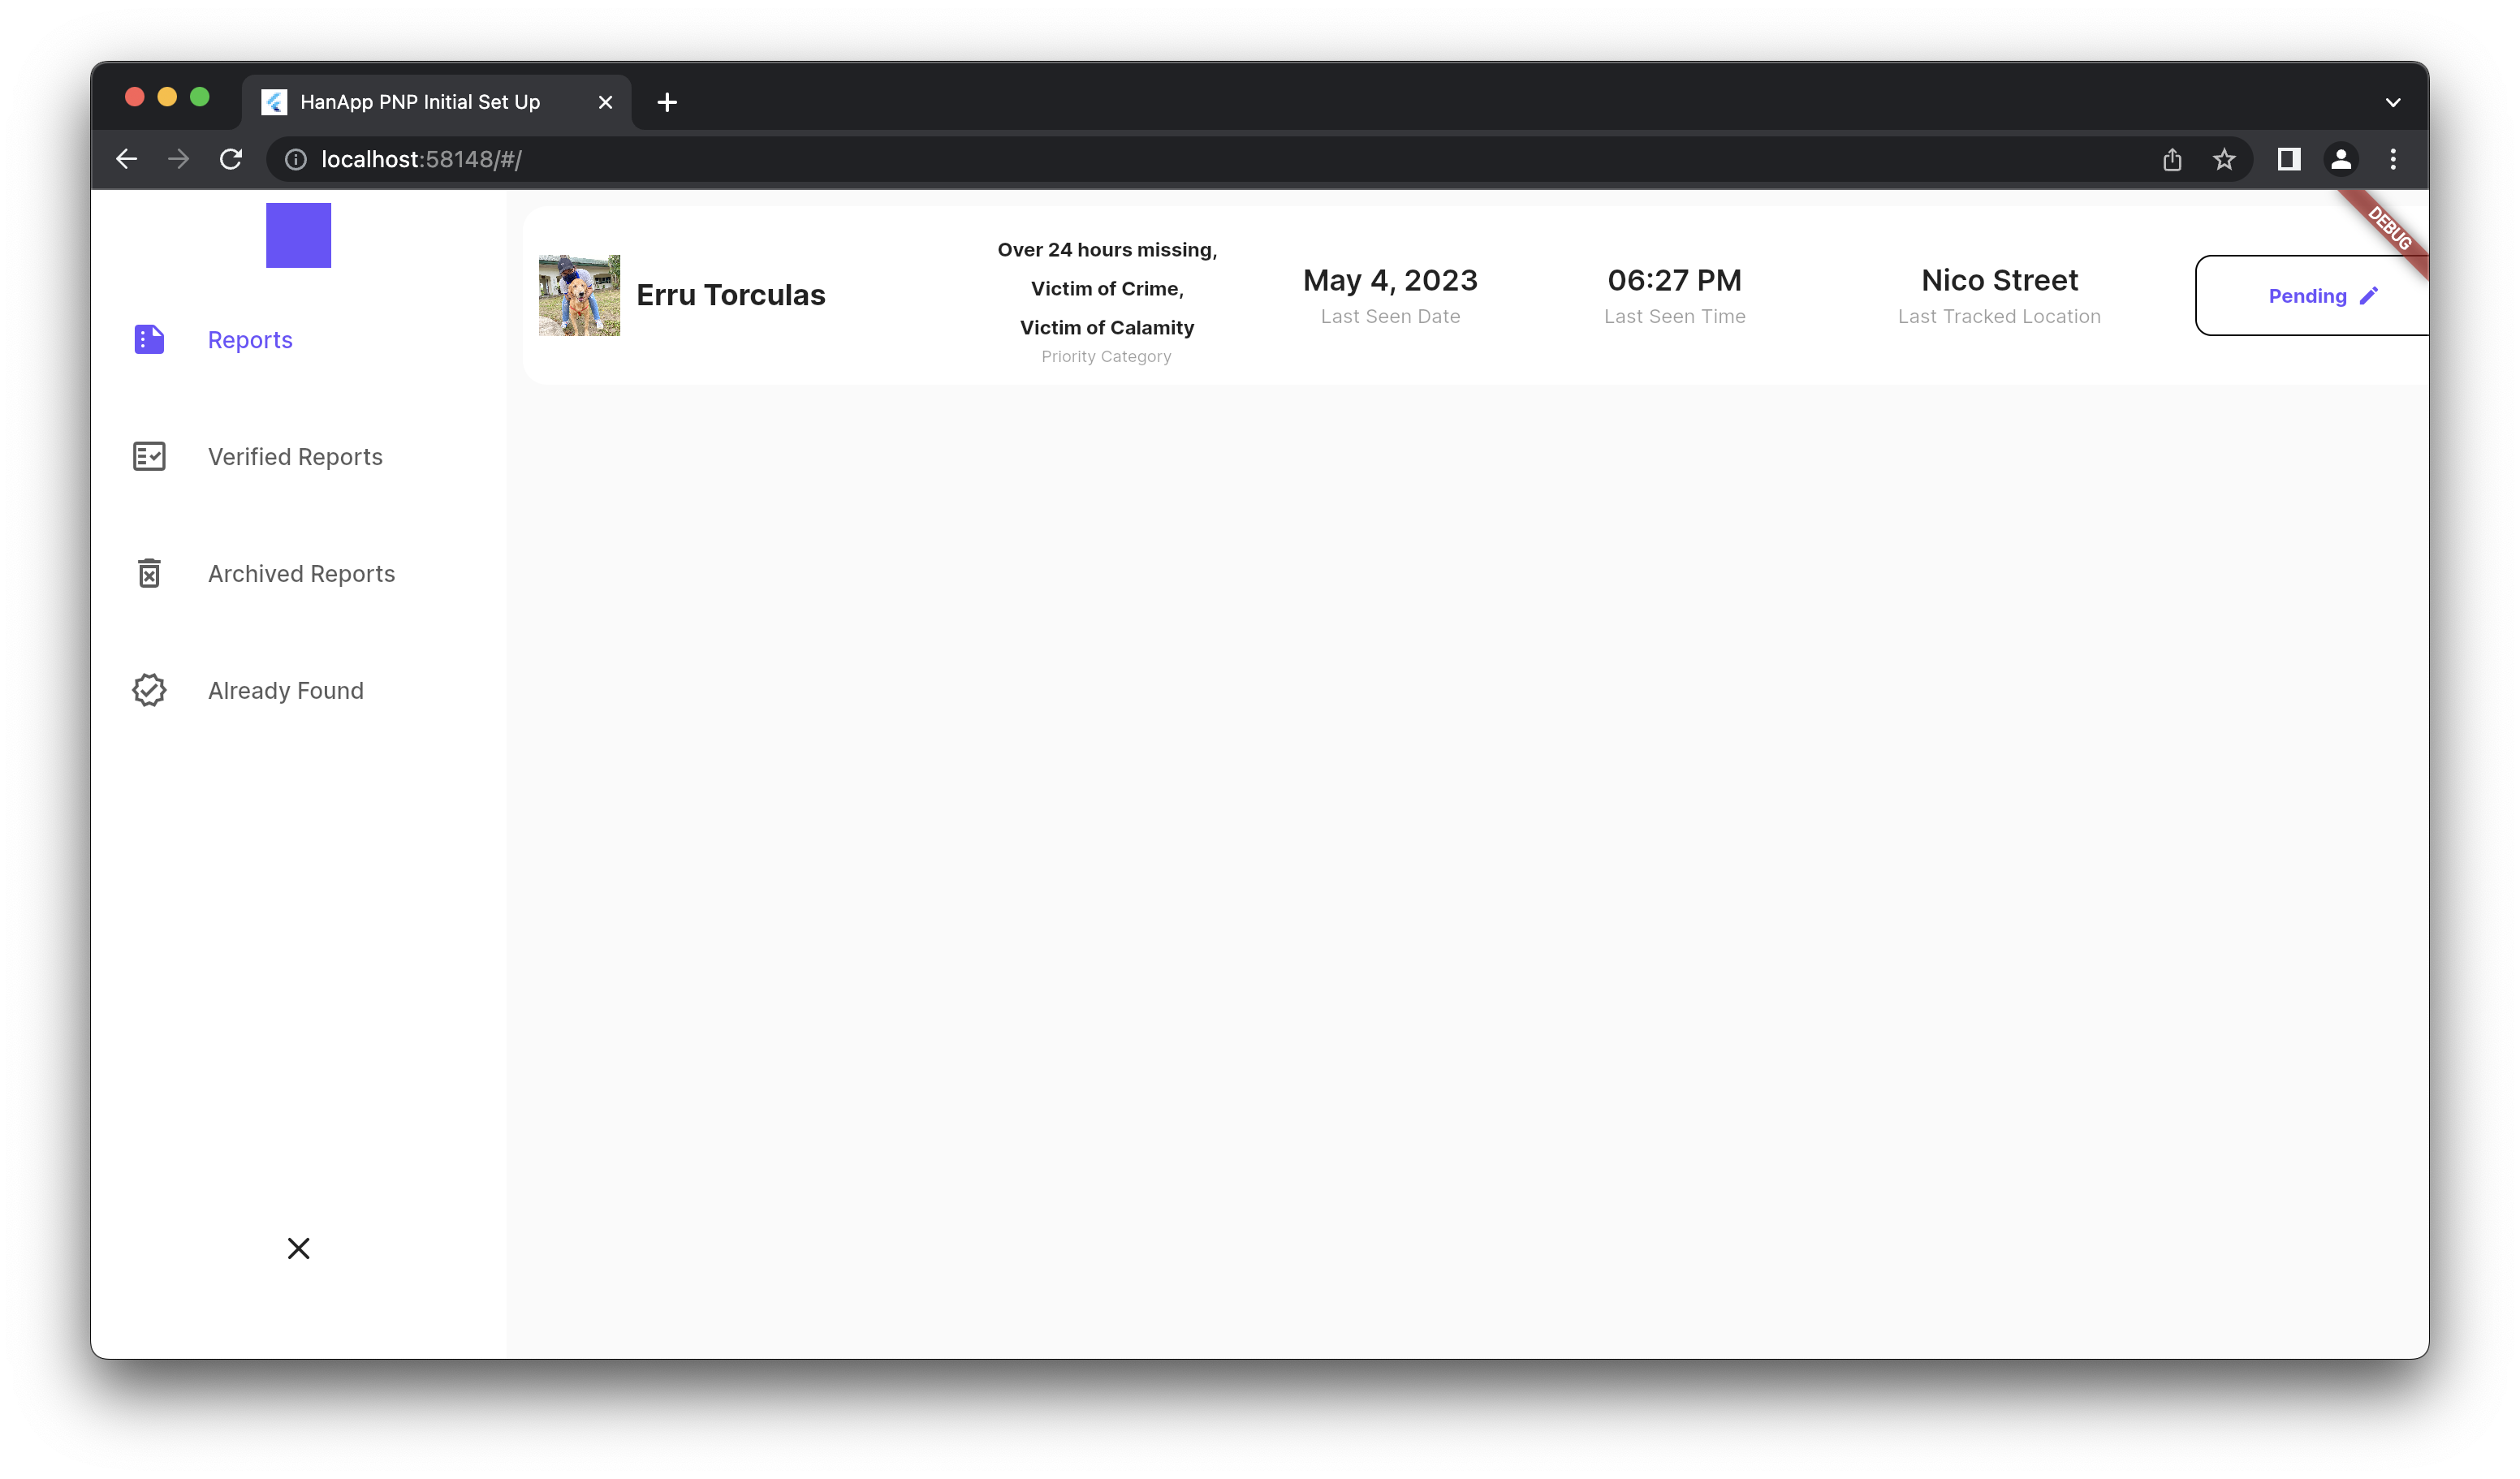
\includegraphics[scale=0.25]{figures/Chapter4/PNP/NavigationTab.png}
    \caption{Admin Reports Management Suite View}
    \label{fig:PNP2}
\end{figure}
\subsection{PNP Admin Reports Management Suite}

Figure \ref{fig:PNP2} is the management suite for the PNP to access reports. The Reports page will have a scrollable list that will consist of the various details such as MP’s name, status of the report, time and date reported, and the location of MP. As for the status, a dropdown menu will be used to categorize each report namely, Received, Already Found, Verify Report, and Reported. For better management, reports are correctly being filtered into their respective statuses onto the different menus as seen on the left-hand side of the interface (i.e. verified reports will be on the verified menu).

\begin{figure}[!h]
    \centering
    \begin{subfigure}[c]{1\linewidth}
        \centering
        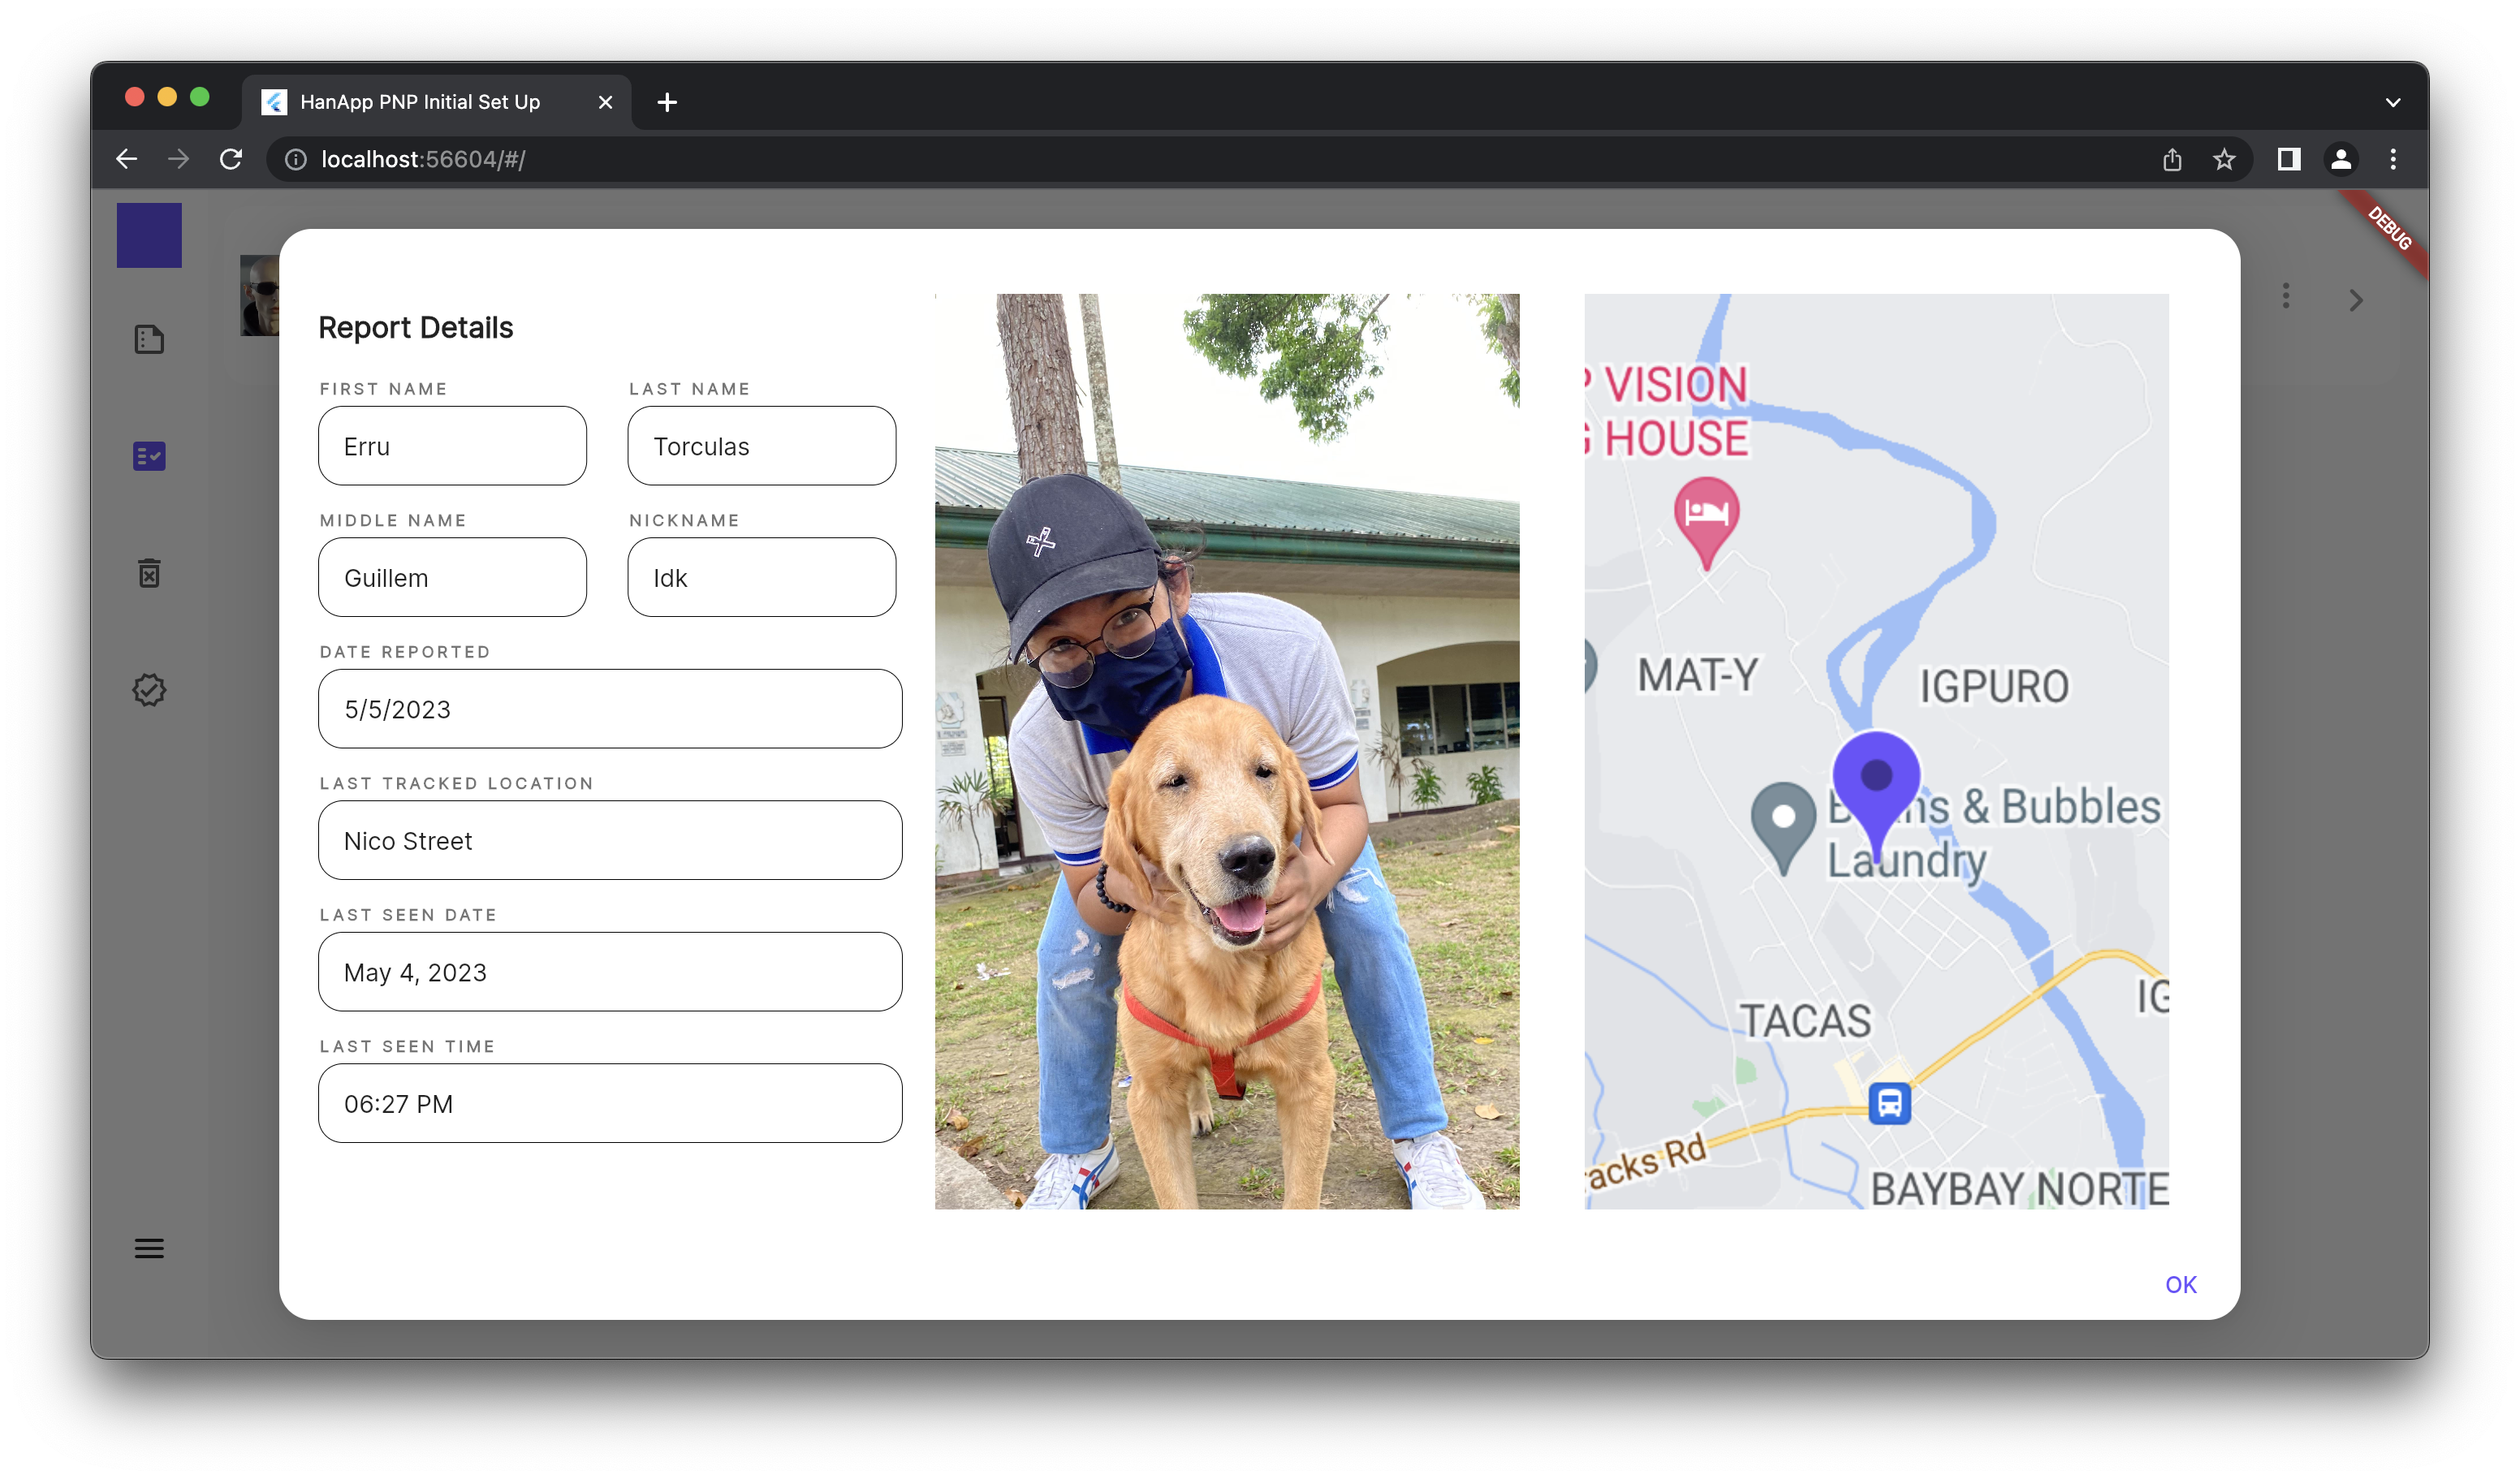
\includegraphics[scale=0.25]{figures/Chapter4/PNP/reportDetails-1.png}
    \end{subfigure}
    \centering
    \begin{subfigure}[c]{1\linewidth}
        \centering
        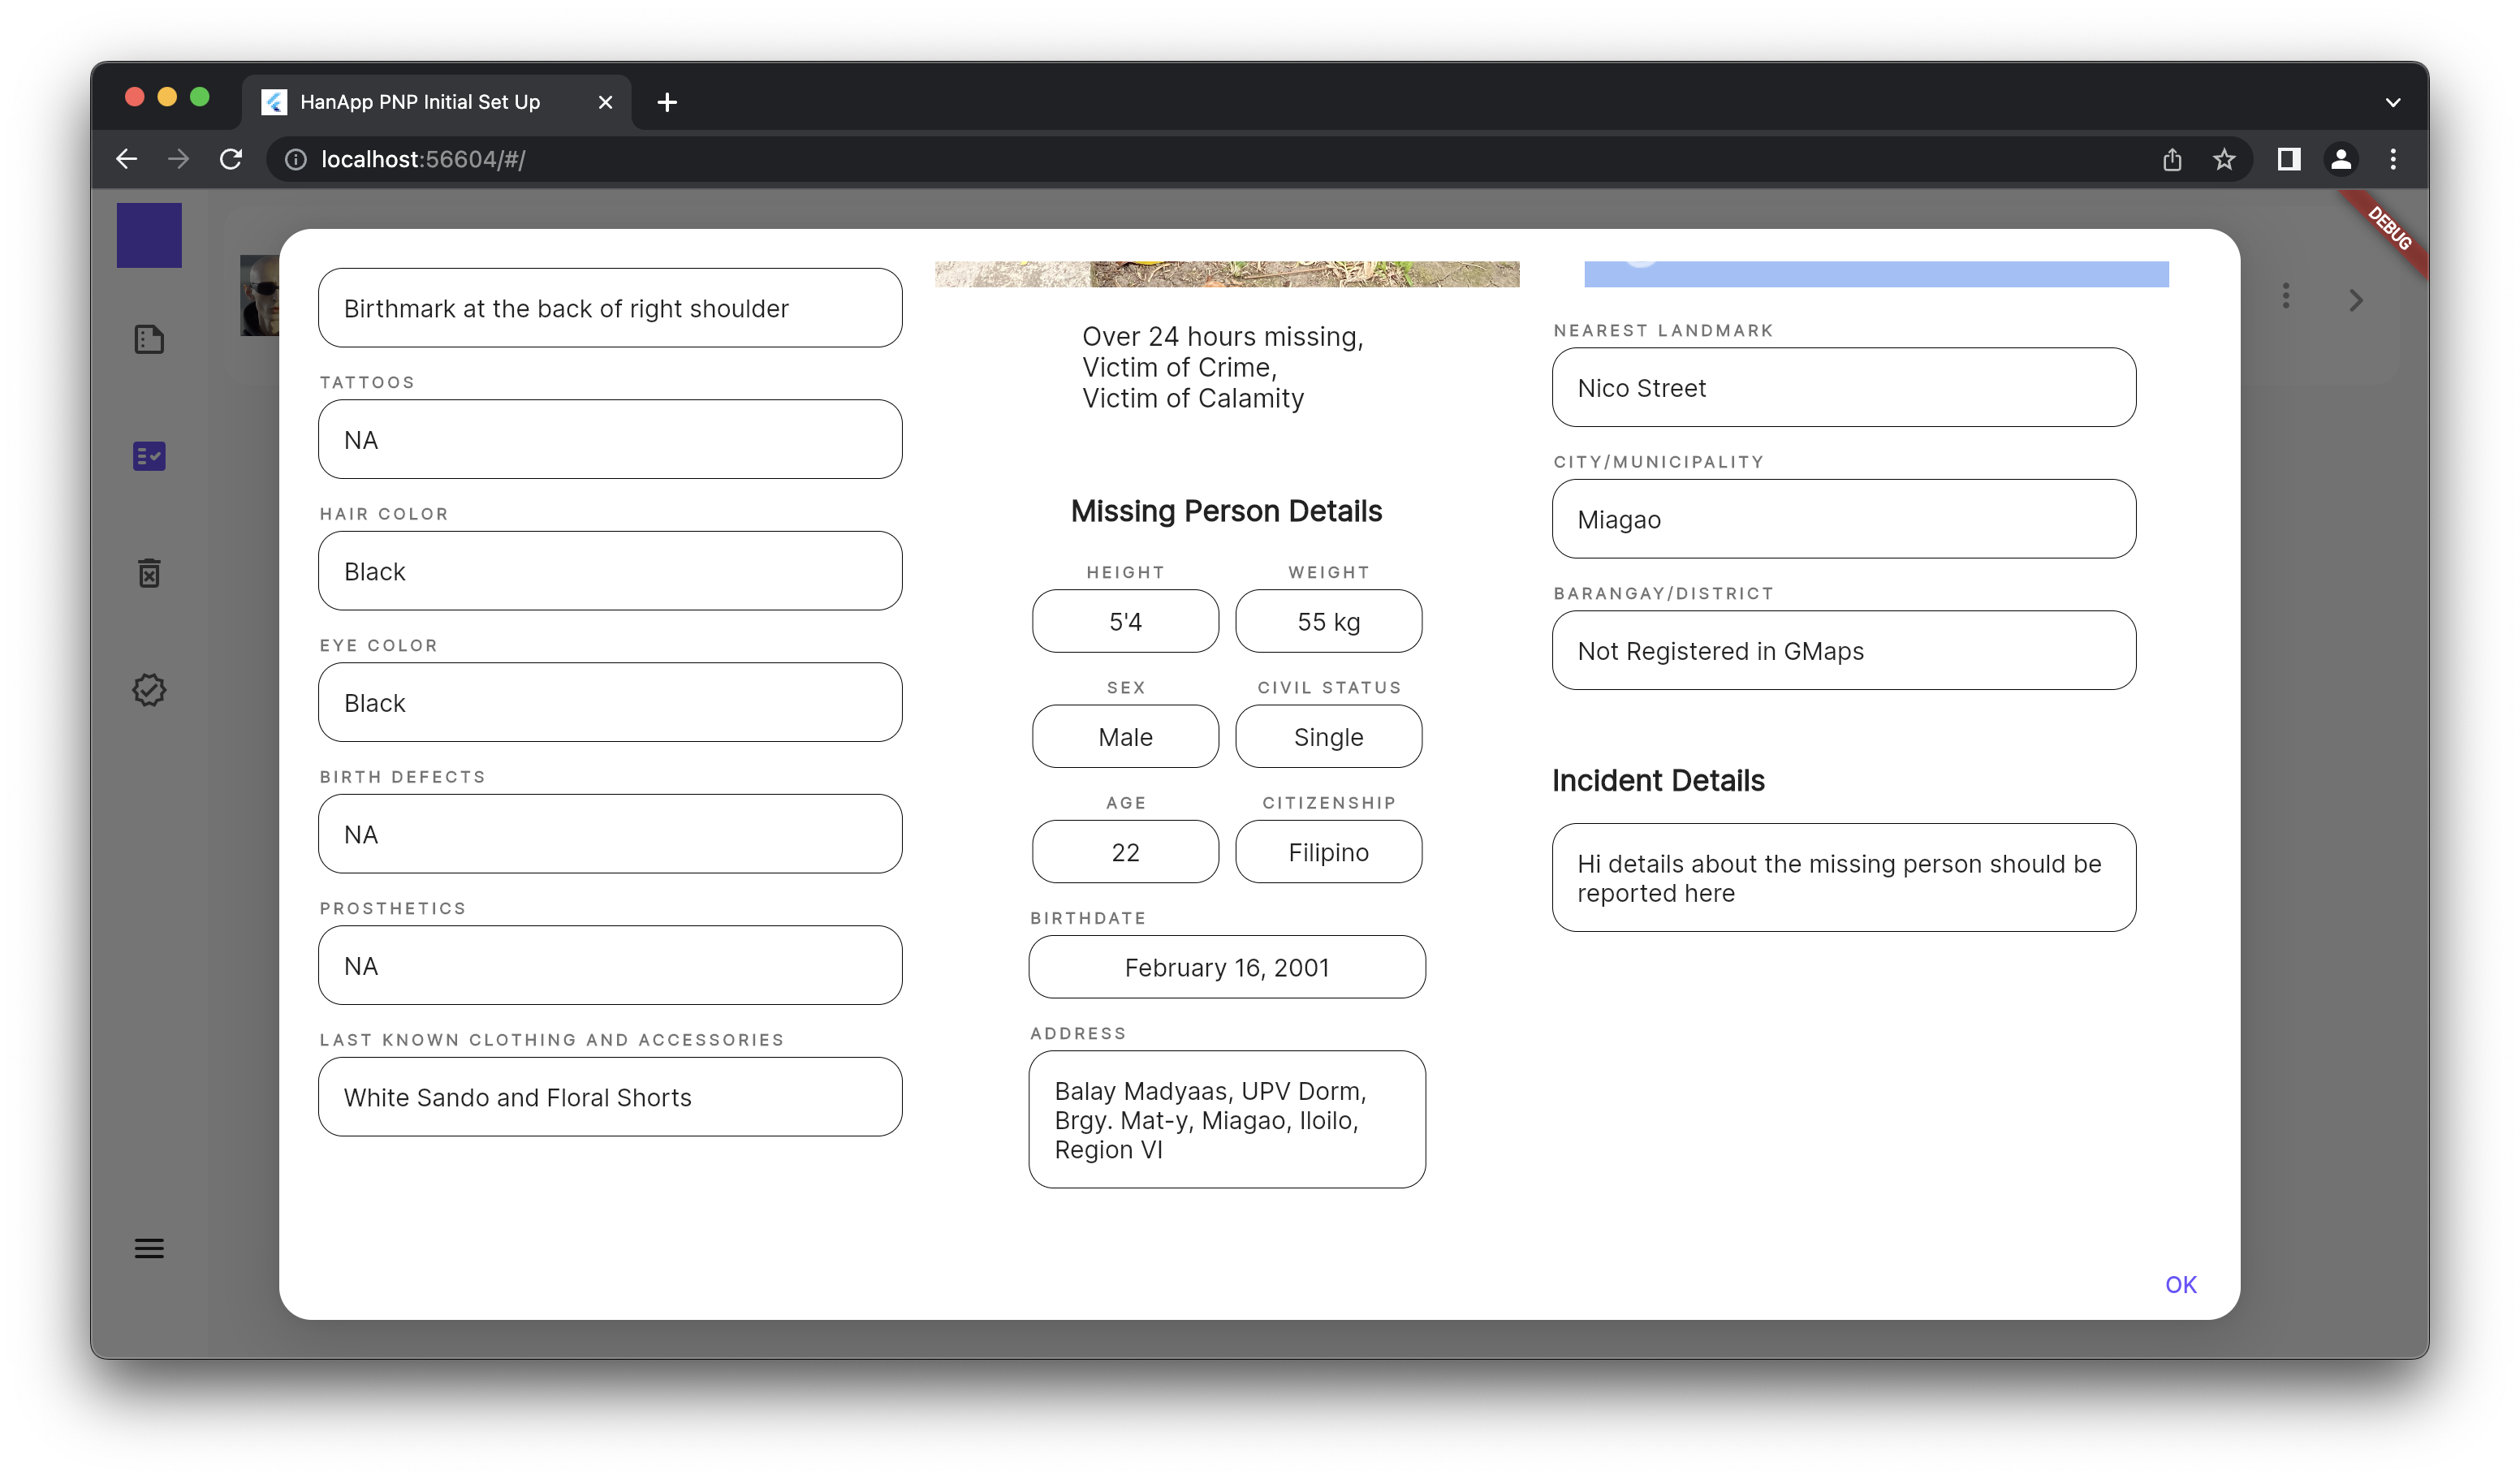
\includegraphics[scale=0.25]{figures/Chapter4/PNP/reportDetails-2.png}
    \end{subfigure}
    \caption{Dialog Box of Report Details}
    \label{fig:reportDetails}
\end{figure}

\subsubsection{Viewing Report Details}

The report dialog box details the list of the necessary information that the reportee provided. Figure \ref{fig:reportDetails} illustrates missing person's descriptions, last seen location snapshot, and their picture that will be shown first to ease the process of identification. It's important to note that these are all the same and exact information required by the PNP when filing or verify a report of the missing person as per their guidelines on handling missing persons cases \cite{NationalPoliceCommission}. But compared to the numerous forms required in their guidelines, the details are more compact and summarized for their convenience. The data can be retrieved from the database through shared preferences plugin used.

\section{User or Main Interface}
The main interface will be subdivided into three various parts to cover all the features that was built throughout the process.

\subsection{User Account Registration, Authentication, and Login}
Authentication is necessary for the user-side. Figures \ref{fig:userLogin} and \ref{fig:userRegister} are the Login and Register page, respectively. Input fields will be provided for the registration such as email address, full name, sex, birth date, and a numeric input field will be observed for the phone number. To ensure that the user understands the Terms and Conditions and Privacy Policy, a hyperlinked text can be used to redirect them for their perusal. Then a register button will let the user account be registered and store in the database for authentication purposes.
\begin{figure}[!h]
    \centering
    \begin{minipage}[c]{0.50\linewidth}
        \centering
        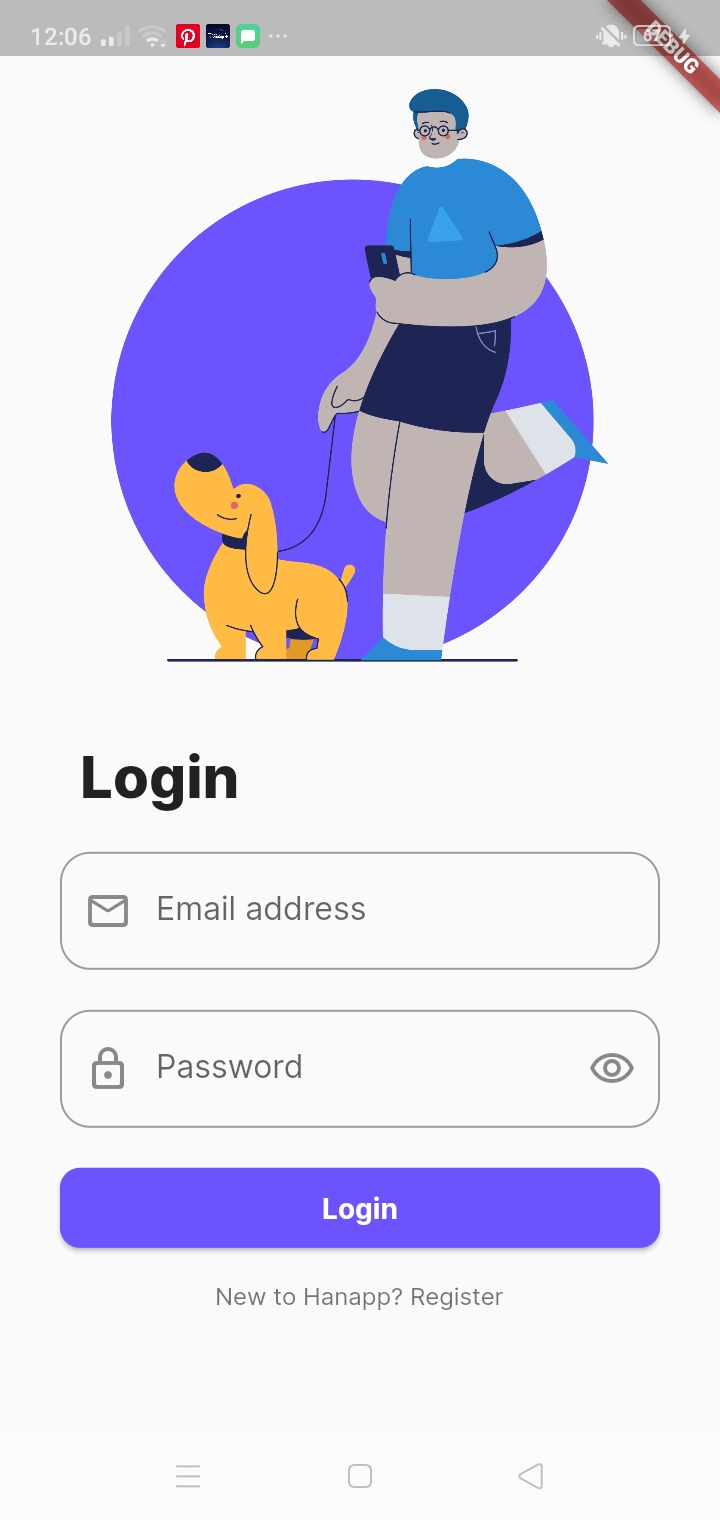
\includegraphics[scale=0.15]{figures/Chapter4/Main/Login.jpg}
        \caption{Login Page}
        \label{fig:userLogin}
    \end{minipage}
\end{figure}

In order to validate the authentication processes, use-case testing was initiated. The functionality of logging in meets the user requirement for a happy path since the expected output was observed. In order to mitigate any erroneous instances of unexpected outcome, incorrect credentials was utilized and as expected, the application will deter these circumstances.

\begin{figure}[!h]
    \centering
    \begin{subfigure}[c]{0.30\linewidth}
        \centering
        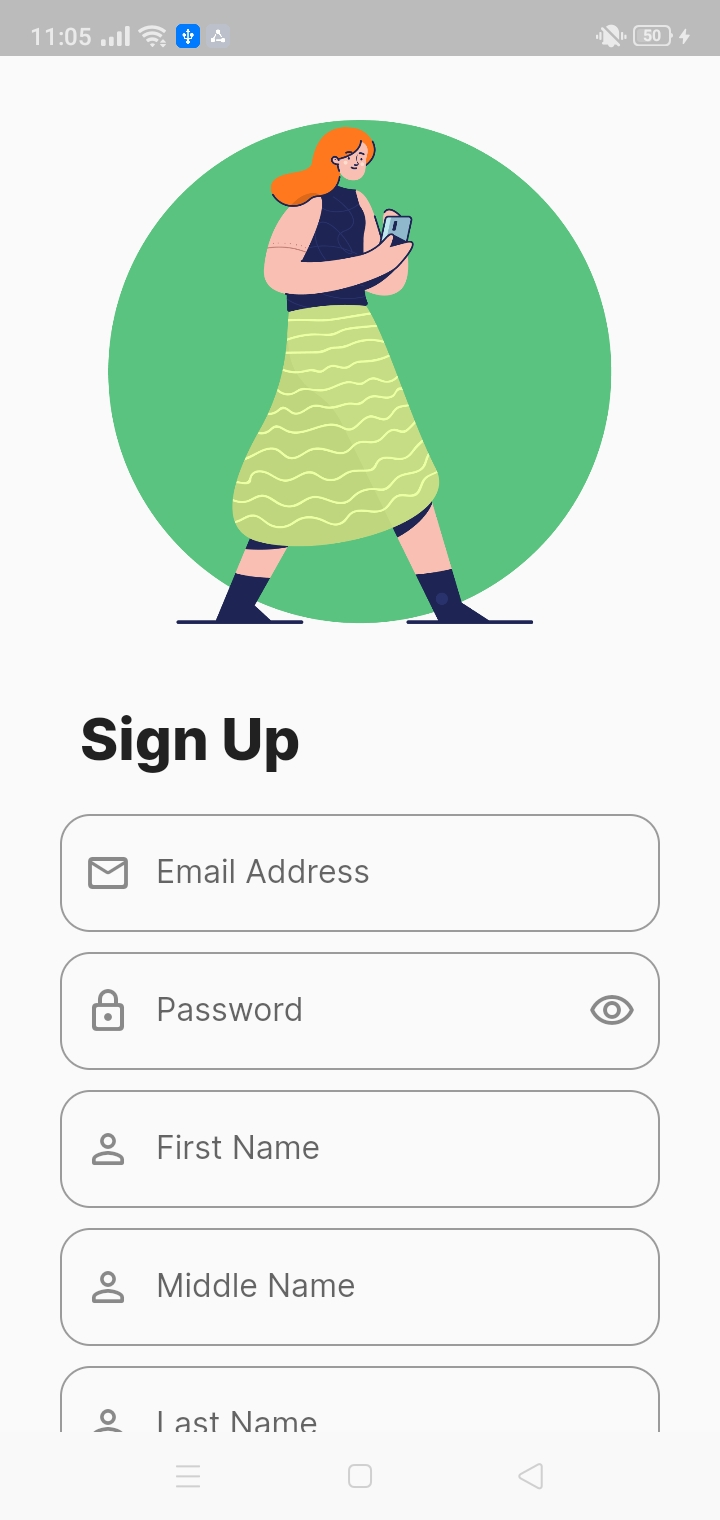
\includegraphics[scale=0.15]{figures/Chapter4/Main/SignUp-1.jpg}
    \end{subfigure}
    \centering
    \begin{subfigure}[c]{0.30\linewidth}
        \centering
        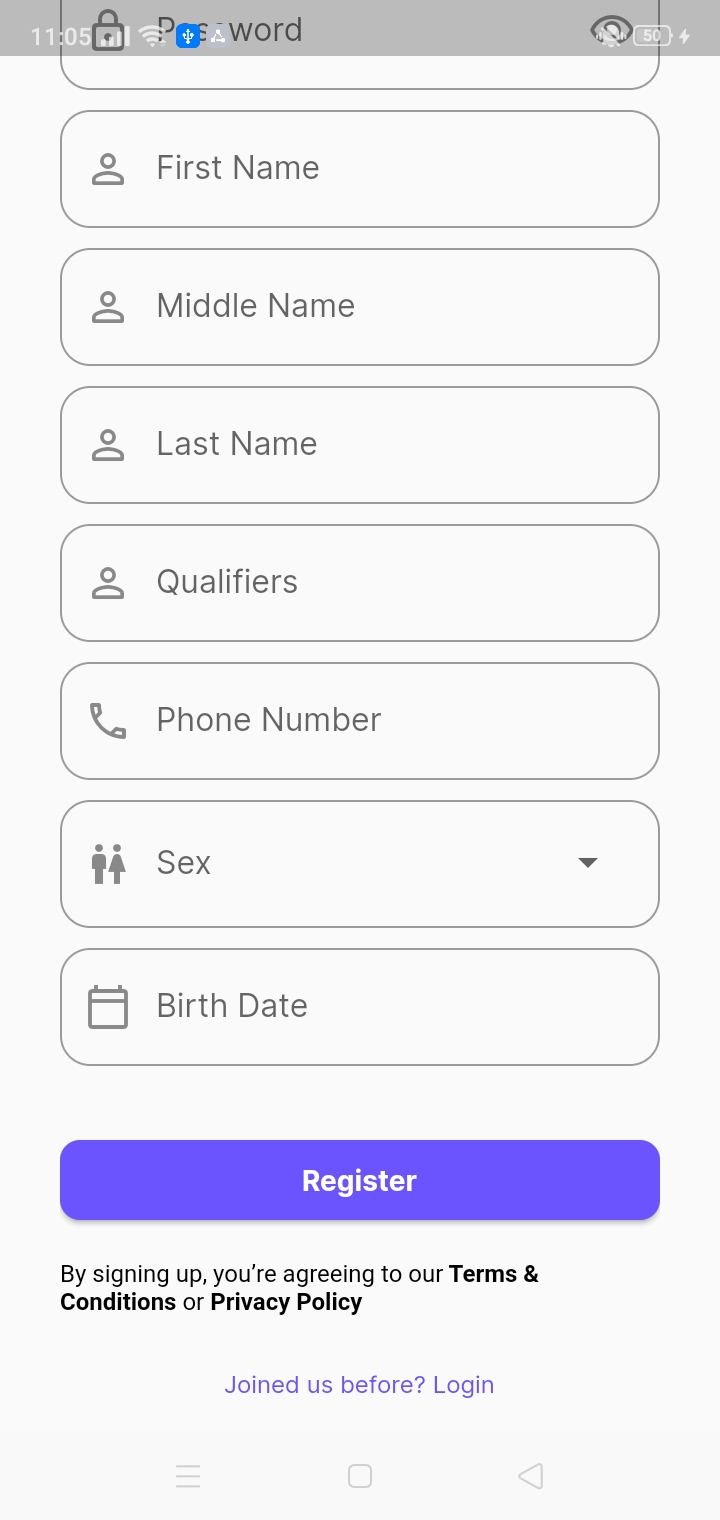
\includegraphics[scale=0.15]{figures/Chapter4/Main/SignUp-2.jpg}
    \end{subfigure}
    \caption{Sign Up Page}
    \label{fig:userRegister}
\end{figure}

\subsubsection{Account Verification}
In order to make sure that newly registered accounts are of human-origin and are legit accounts of potential users, accounts need to be authenticated first before being able to login. Figure \ref{fig:accountVerification}   illustrates the process of verification: first, after the user is registered, they will be redirected to a page where they will be given the choice to send email verification onto their newly registered email address for the application, or to redirect to the login page instead. If users select the option to send the verification email, they can then check their respective emails that ask for verification that, after clicking the link in the email, would mark their registered accounts as verified, allowing them to be able to login. If in some cases that users will opt-out of sending the verification email right after being registered, they still will be met with the same verification page if they try to login with a none email-verified account. 
\begin{figure}[!h]
    \centering
    \begin{subfigure}[c]{0.30\linewidth}
        \centering
        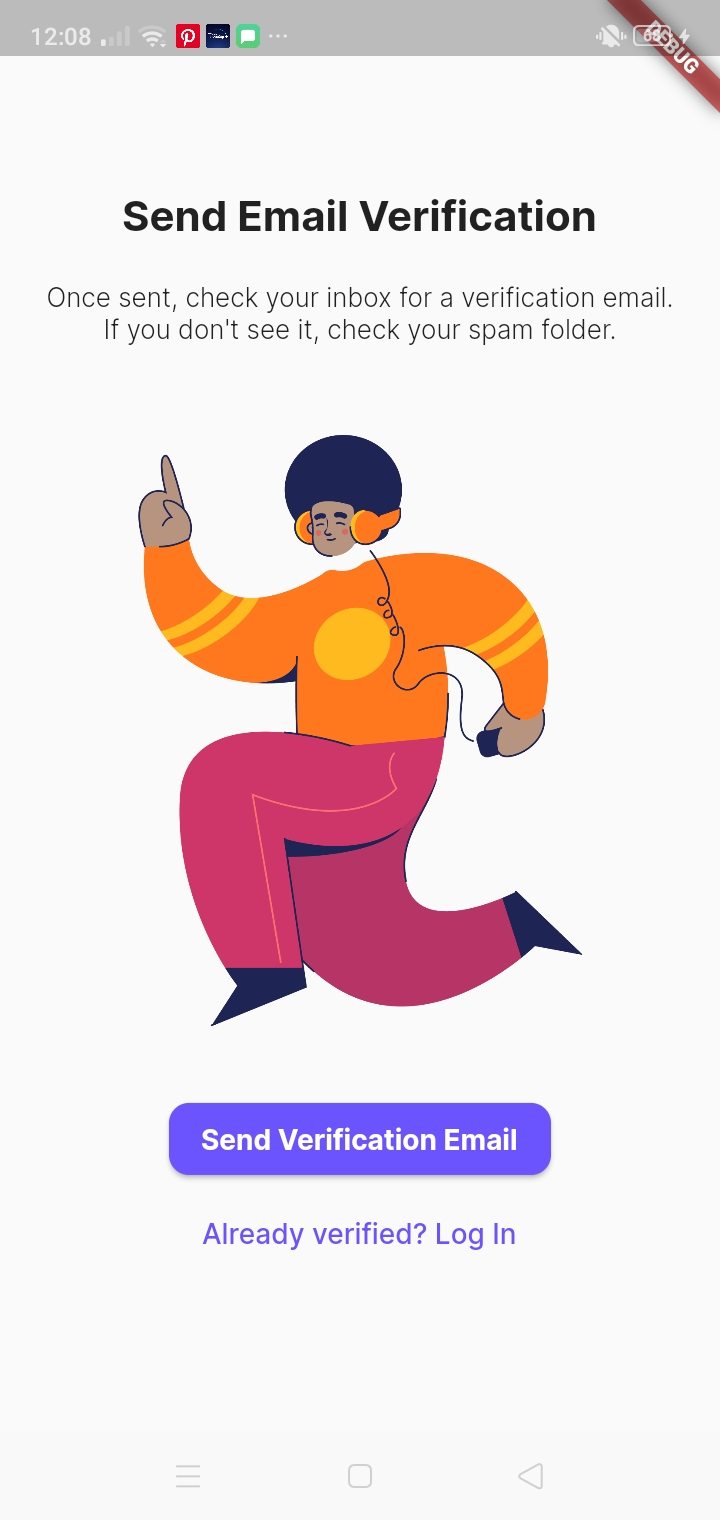
\includegraphics[scale=0.15]{figures/Chapter4/Main/Verification-1.jpg}
    \end{subfigure}
    \centering
    \begin{subfigure}[c]{0.30\linewidth}
        \centering
        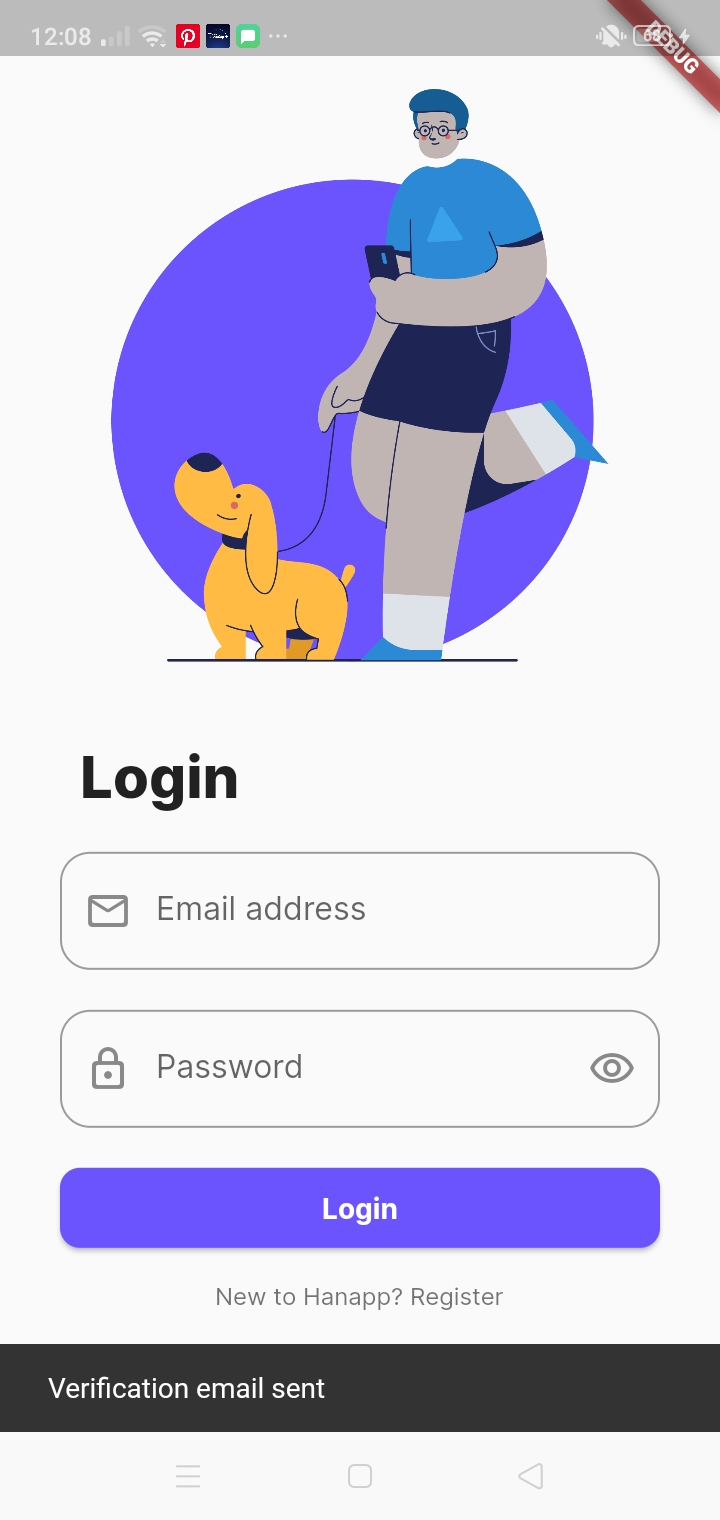
\includegraphics[scale=0.15]{figures/Chapter4/Main/Verification-4.jpg}
    \end{subfigure}
    \centering
    \begin{subfigure}[c]{0.30\linewidth}
        \centering
        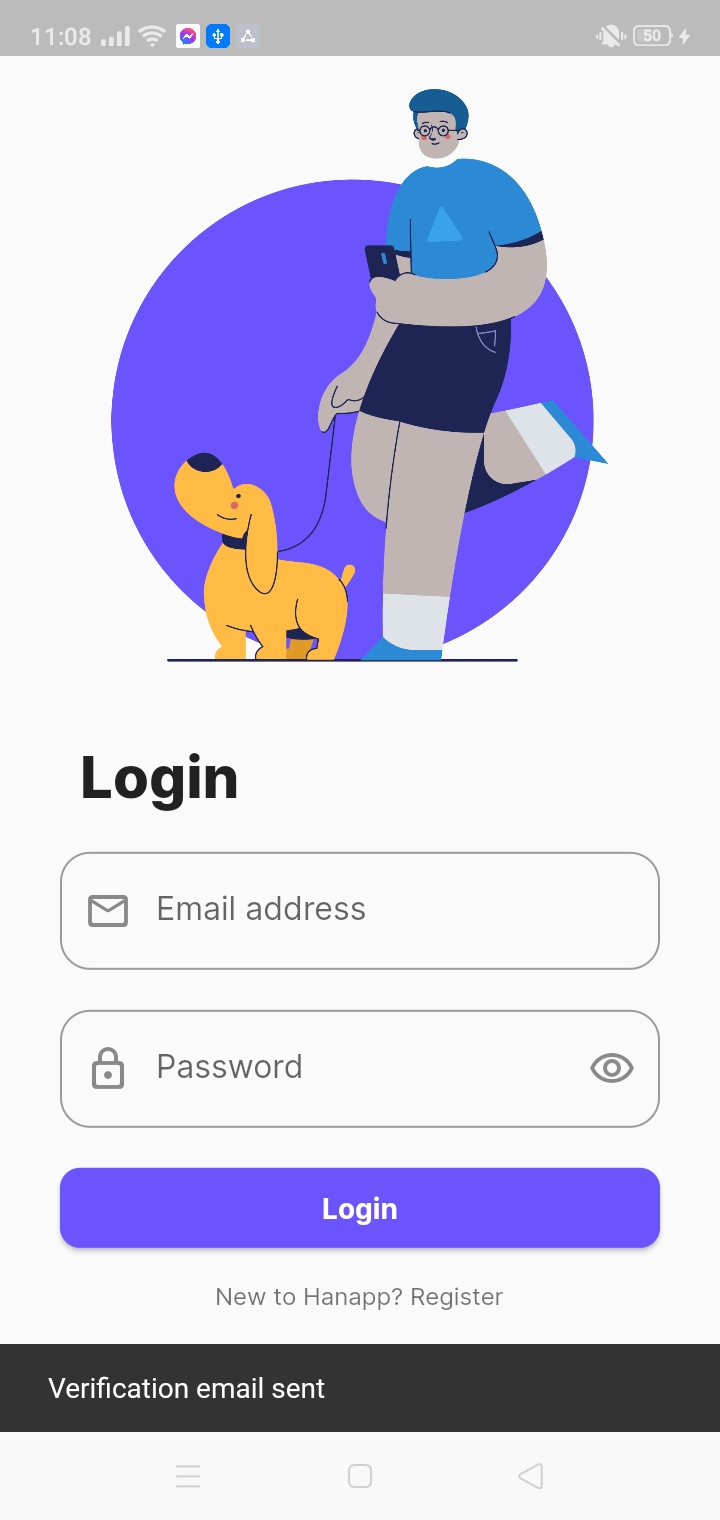
\includegraphics[scale=0.15]{figures/Chapter4/Main/Verification-2.jpg}
    \end{subfigure}
    \caption{Account Verification Process}
    \label{fig:accountVerification}
\end{figure}

\begin{figure}[!h]
    \centering
    \begin{minipage}[c]{0.40\linewidth}
        \centering
        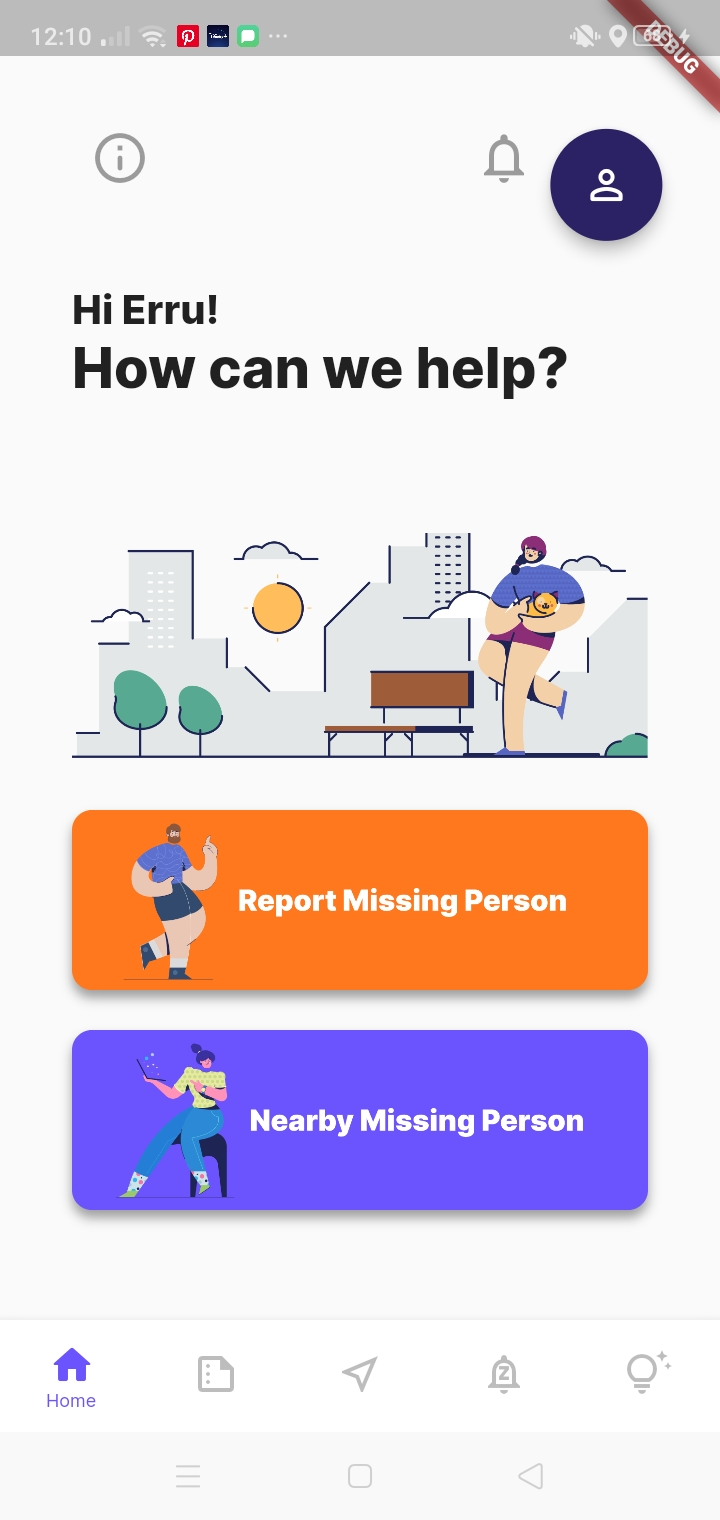
\includegraphics[scale=0.15]{figures/Chapter4/Main/Home.jpg}
        \caption{Home Page}
        \label{fig:userHome}
    \end{minipage}
    \centering
    \begin{minipage}[c]{0.40\linewidth}
        \centering
        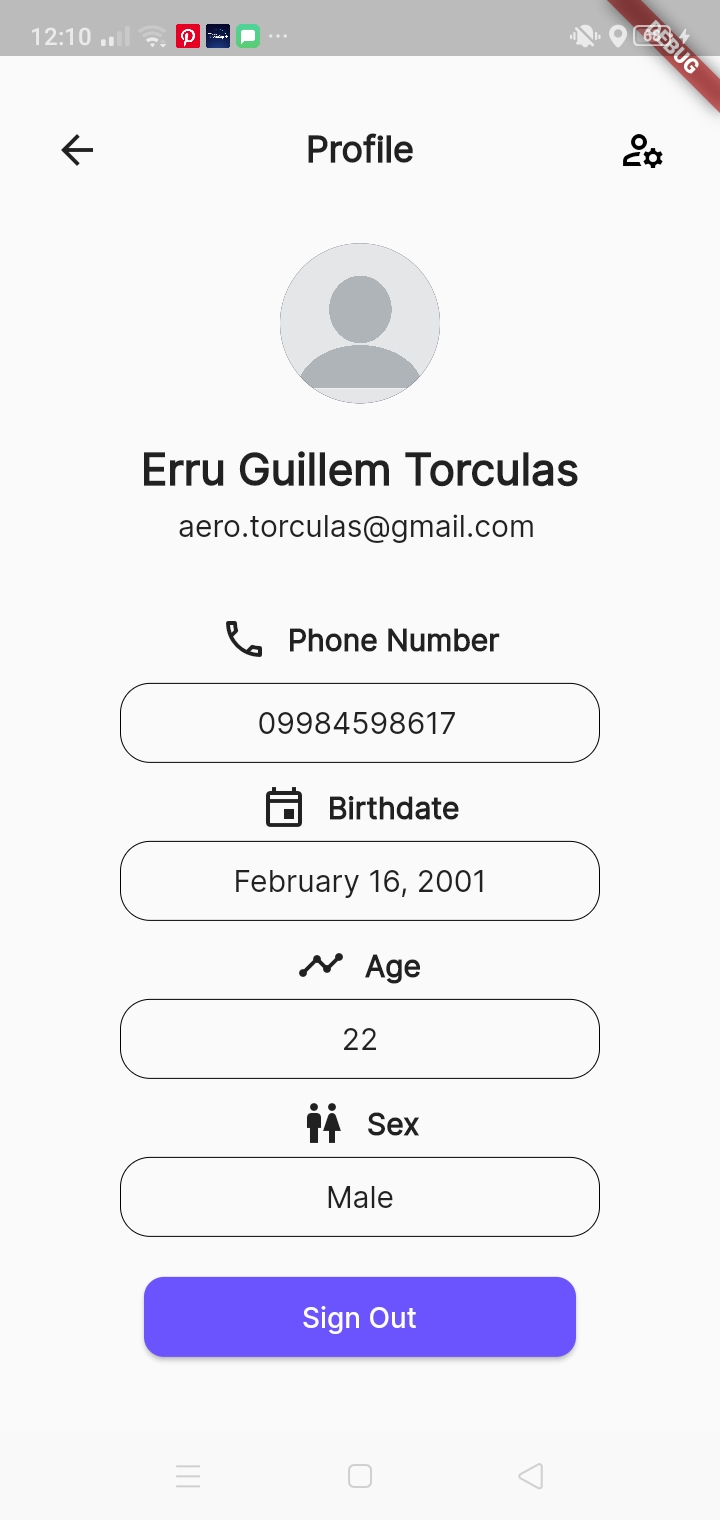
\includegraphics[scale=0.15]{figures/Chapter4/Main/Profile.jpg}
        \caption{Profile Page}
        \label{fig:userProfile}
    \end{minipage}
\end{figure}
Moreover, when user authentication is completed, the login button will let them proceed to the Home page of the application where the user will have two options: Report Missing or Nearby Missing persons as shown in \ref{fig:userHome}. This will allow the user to optimally choose what course of action are they going to take on by presenting these call to action button first. A bottom navigation bar will be visible throughout the user’s interaction of the app assuring that they can easily navigate the entire features offered to them. The navigation bar will consist of five (5) sections, namely, Home, Reports, Nearby, Notifications, and Updates. Each section will be utilized to build the features of the app and functions specifically to the needs of the user. \ref{fig:userProfile} illustrates the profile page that will consist of the details about the user that was already pre-filled on the registration part. Thus, it will display: the concatenated full name of the user, email address used in account registration, birth-date, age, and lastly sex. In addition, a sign out button will also be provided in case the user decided to log out from their account.


\subsection{Report Pages}

The Report page is one of the integral parts of this application that would allow users to give necessary information in the event of a person missing. It streamlines the reporting process done by the PNP and replicates their incident report, one that had to be done in written format in their respective outposts, so that verification is manageable \cite{NationalPoliceCommission}. Input text fields will be used throughout this page. Accompanying it with dropdown menus for categorical information such as Gender, and Blood type. Physical indicators will have mostly text/paragraph input fields for elaborations and additional details that are needed to disclose such as body marks, tattoos, and the like.

\begin{figure}[!h]
    \centering
    \begin{minipage}[c]{0.50\linewidth}
        \centering
        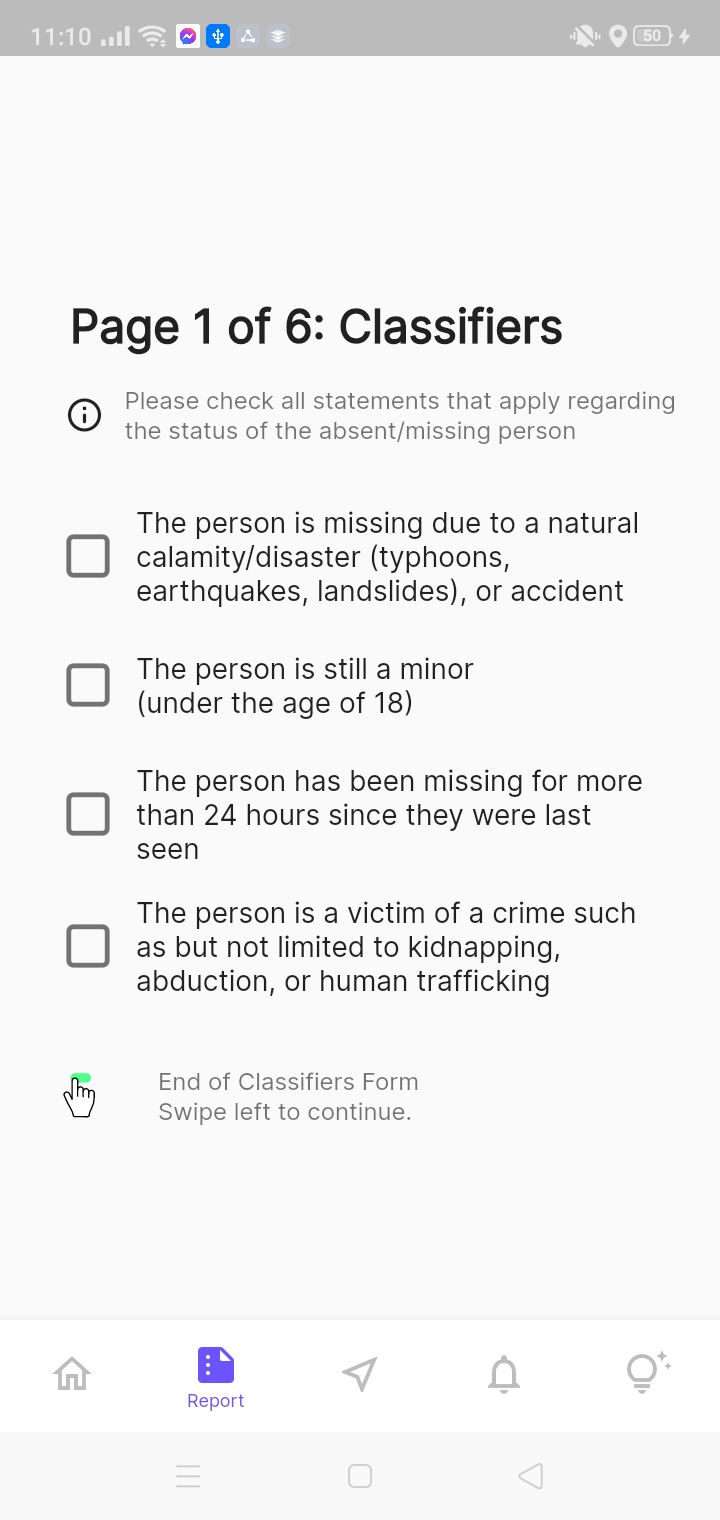
\includegraphics[scale=0.15]{figures/Chapter4/Main/p1.jpg}
        \caption{Report Form Page 1}
        \label{fig:p1}
    \end{minipage}
\end{figure}

\subsubsection{Report Page 1: Classifiers}

On the first page of the reports section as seen in figure \ref{fig:p1}, the categorization of the missing person being reported is located. The reporting user will be met with checkboxes indicating that their person being reported is (1) a person missing due to natural calamities, (2) a person under the age of 18, and is therefore classified as a minor, (3) a person that has been missing for over 24 hours already, or lastly, (4) a person that is a victim of a crime such as, but not limited to, kidnapping, human trafficking, etc.
\begin{figure}[!h]
    \centering
    \begin{subfigure}[c]{0.30\linewidth}
        \centering
        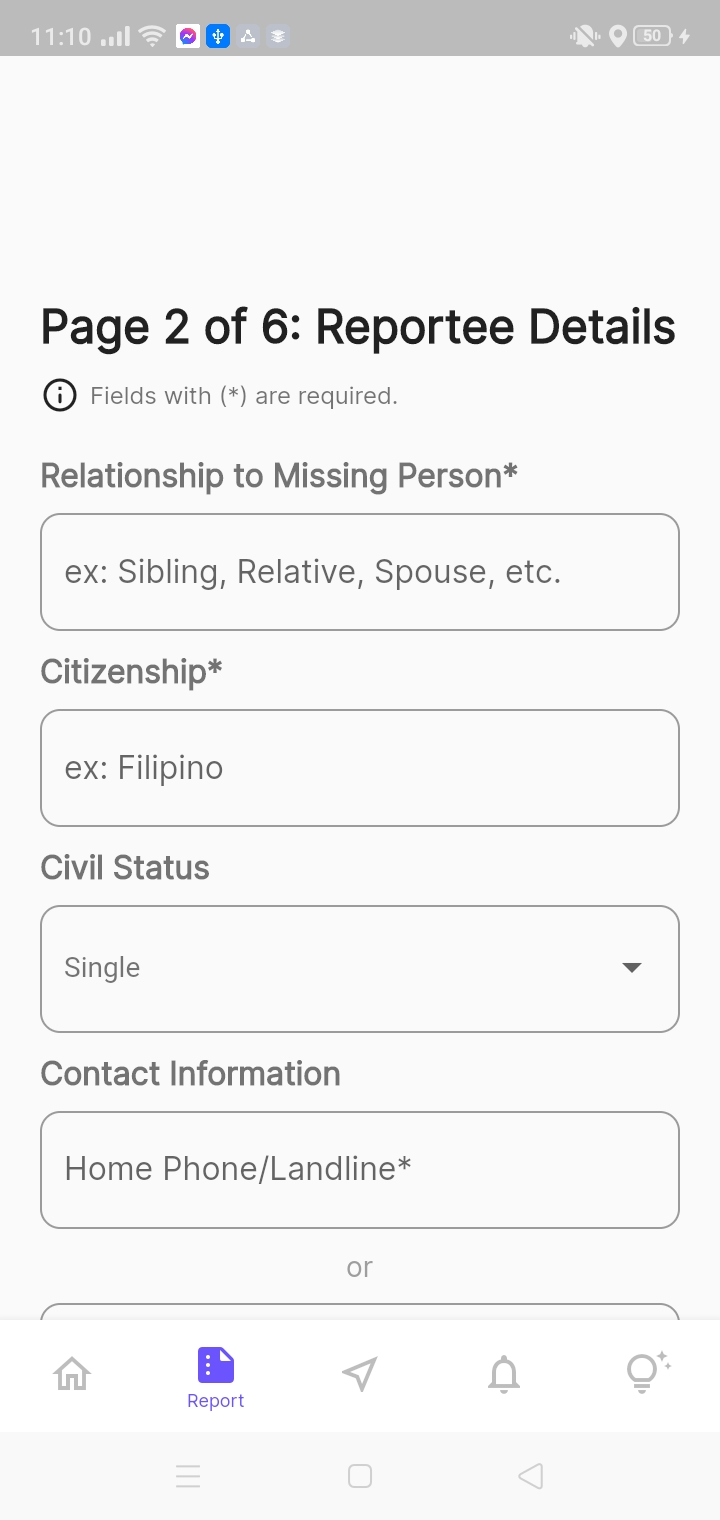
\includegraphics[scale=0.15]{figures/Chapter4/Main/p2-1.jpg}
    \end{subfigure}
    \centering
    \begin{subfigure}[c]{0.30\linewidth}
        \centering
        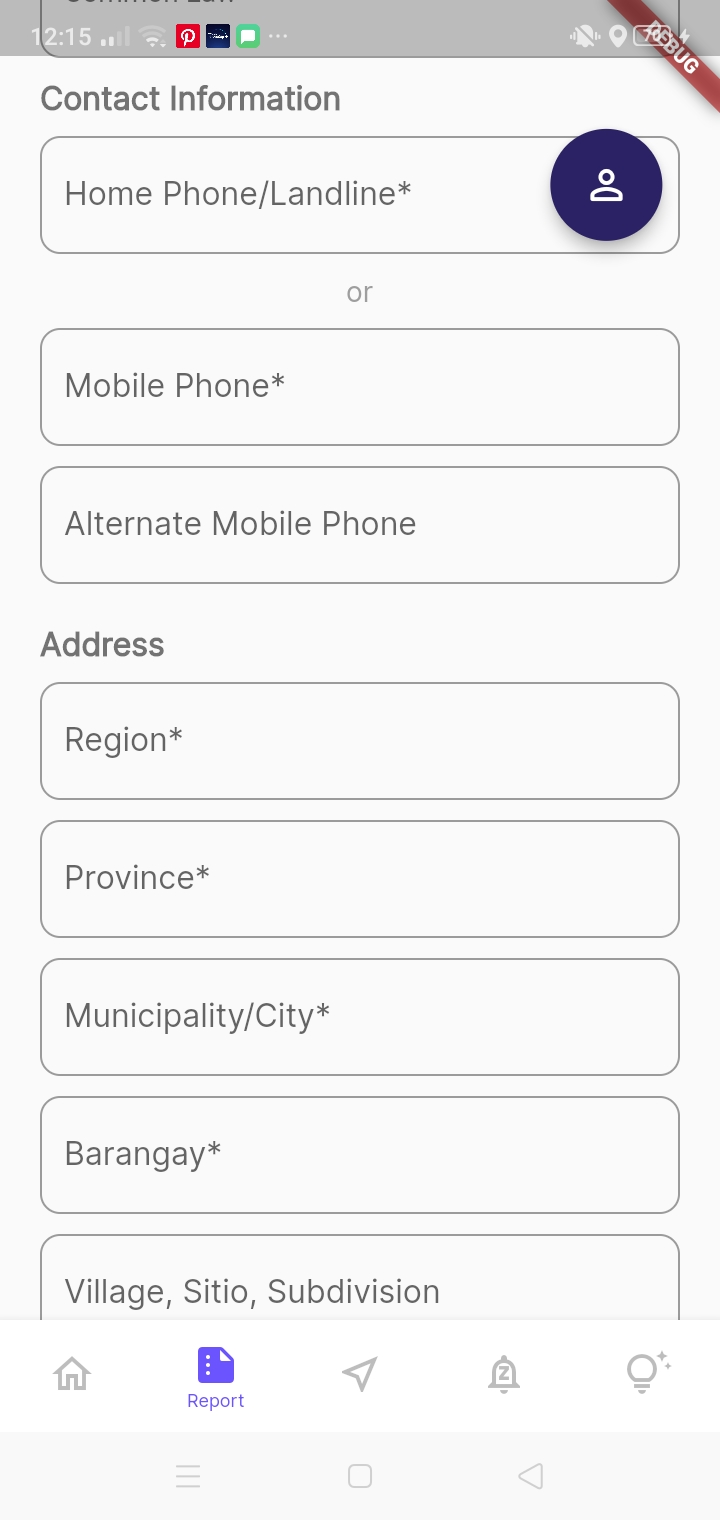
\includegraphics[scale=0.15]{figures/Chapter4/Main/p2-2.jpg}
    \end{subfigure}
    \centering
    \begin{subfigure}[c]{0.30\linewidth}
        \centering
        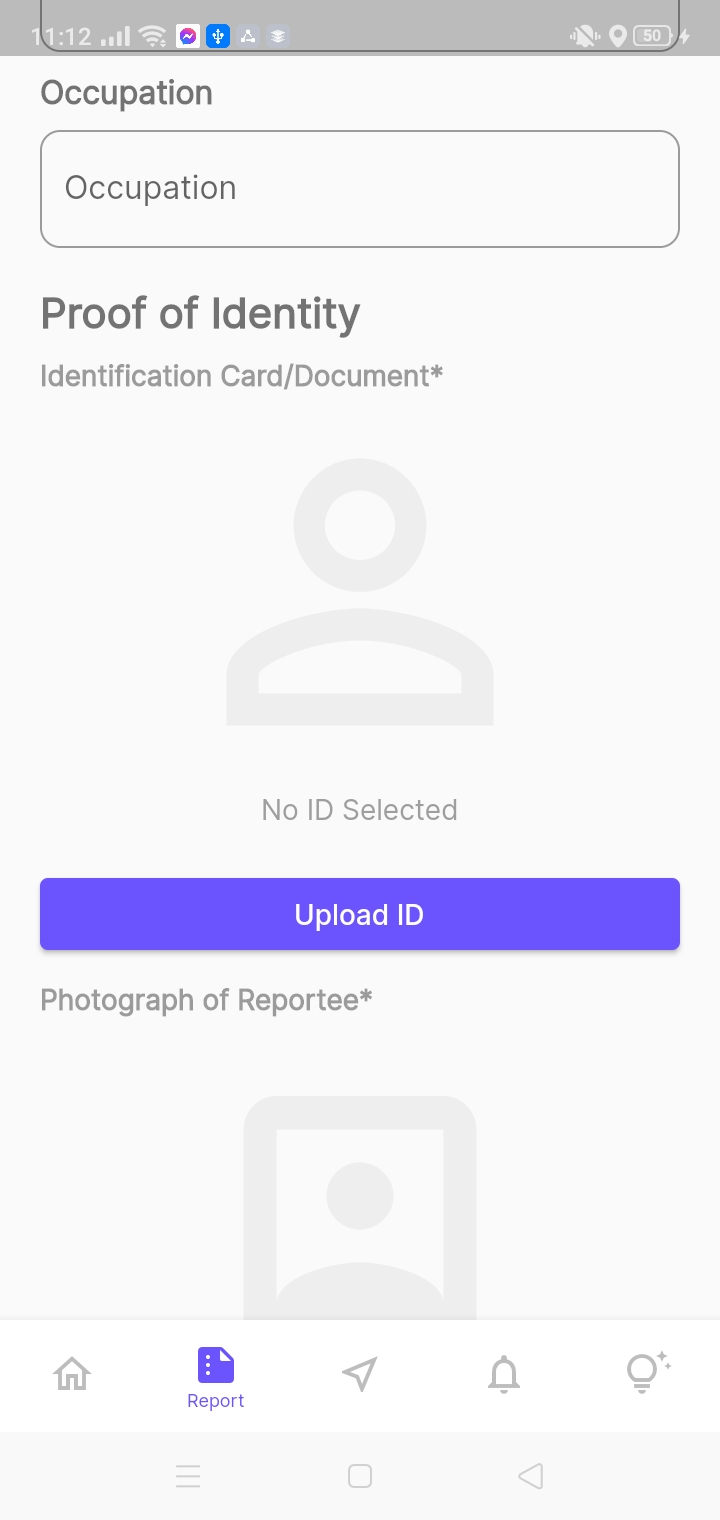
\includegraphics[scale=0.15]{figures/Chapter4/Main/p2-3.jpg}
    \end{subfigure}
    \caption{Report Form Page 2}
    \label{fig:ReportPage2}
\end{figure}
\subsubsection{Report Page 2: Reportee Details}

On the second page of the reports page, as seen in figure \ref{fig:ReportPage2}, the reportee will be asked to fill out required information about them. This includes the reportee's relationship to the missing person, contact information, address, citizenship, and the proofs of identity through a picture of his/her identification card (ID), and a selfie. The selfie serves as a secondary authentication measure in lieu of reporting remotely rather than in person, and also allows the PNP to verify if the user's face matches that of the photo in their submitted ID. The reportee's basic information such as name, birth-date, age, and sex are no longer required to be re-entered since they are now already found in the user's profile. 

\subsubsection{Report Page 3: Absent/Missing Person Details}

The third page of the reports section, as seen in figure \ref{fig:ReportPage3}, requires the necessary information about the reported missing person such as their name, birth-date, sex, address, and contact information. It's important to note the specific usage of the term "Absent/Missing Person" as it is the same term used in PNP's required forms when handling missing persons cases, specifically "Annex C: Checklist for Absent/Missing Person".
\begin{figure}[!h]
    \centering
    \begin{subfigure}[c]{0.30\linewidth}
        \centering
        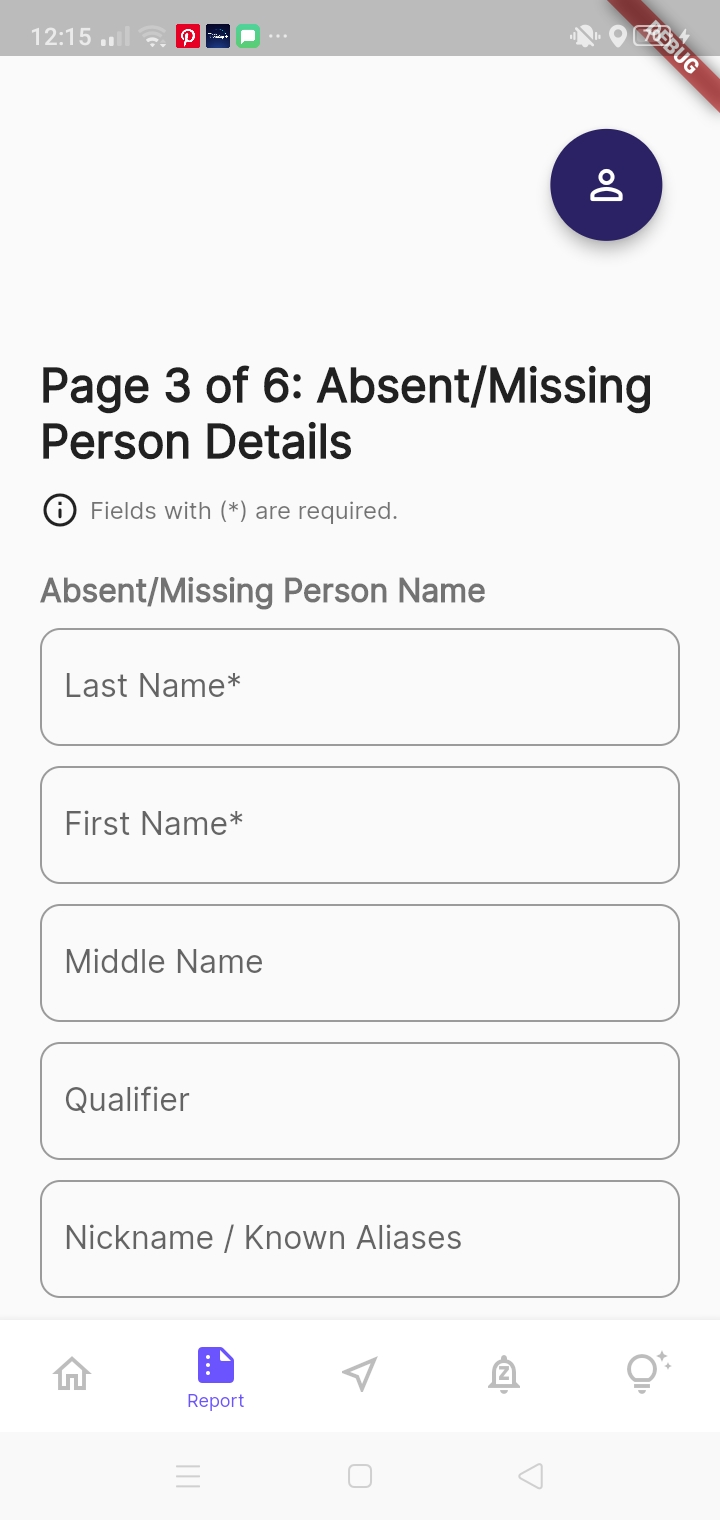
\includegraphics[scale=0.15]{figures/Chapter4/Main/p3-1.jpg}
    \end{subfigure}
    \centering
    \begin{subfigure}[c]{0.30\linewidth}
        \centering
        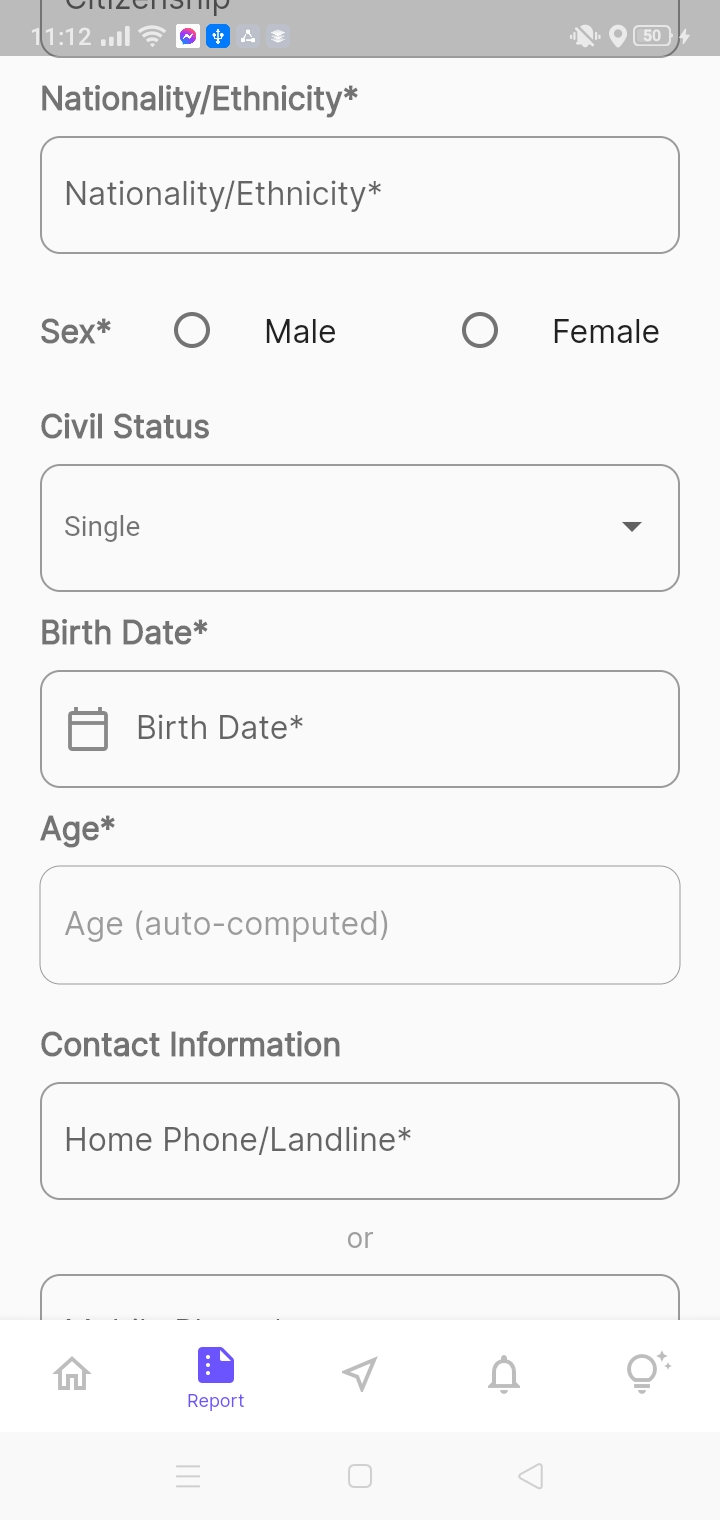
\includegraphics[scale=0.15]{figures/Chapter4/Main/p3-2.jpg}
    \end{subfigure}
    \centering
    \begin{subfigure}[c]{0.30\linewidth}
        \centering
        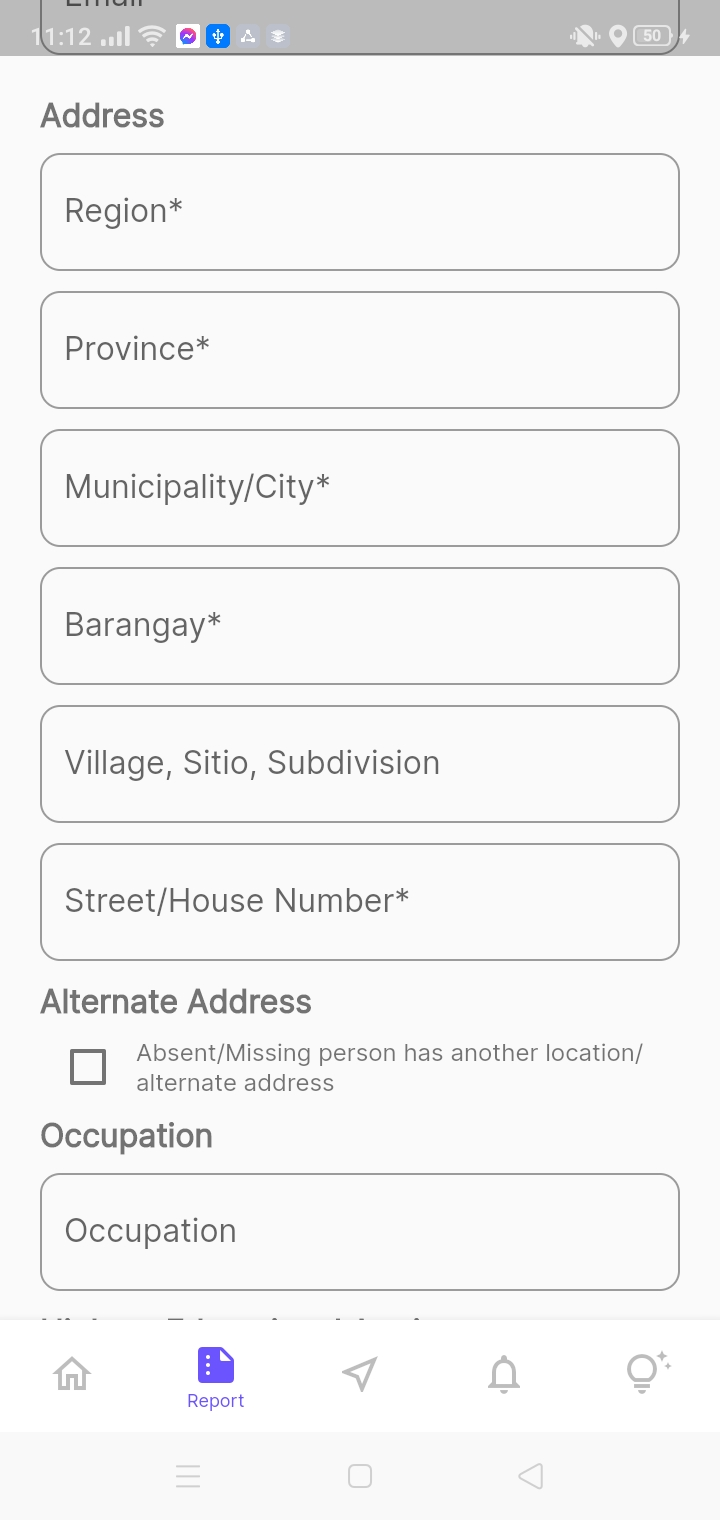
\includegraphics[scale=0.15]{figures/Chapter4/Main/p3-3.jpg}
    \end{subfigure}
        \centering
    \begin{subfigure}[c]{0.30\linewidth}
        \centering
        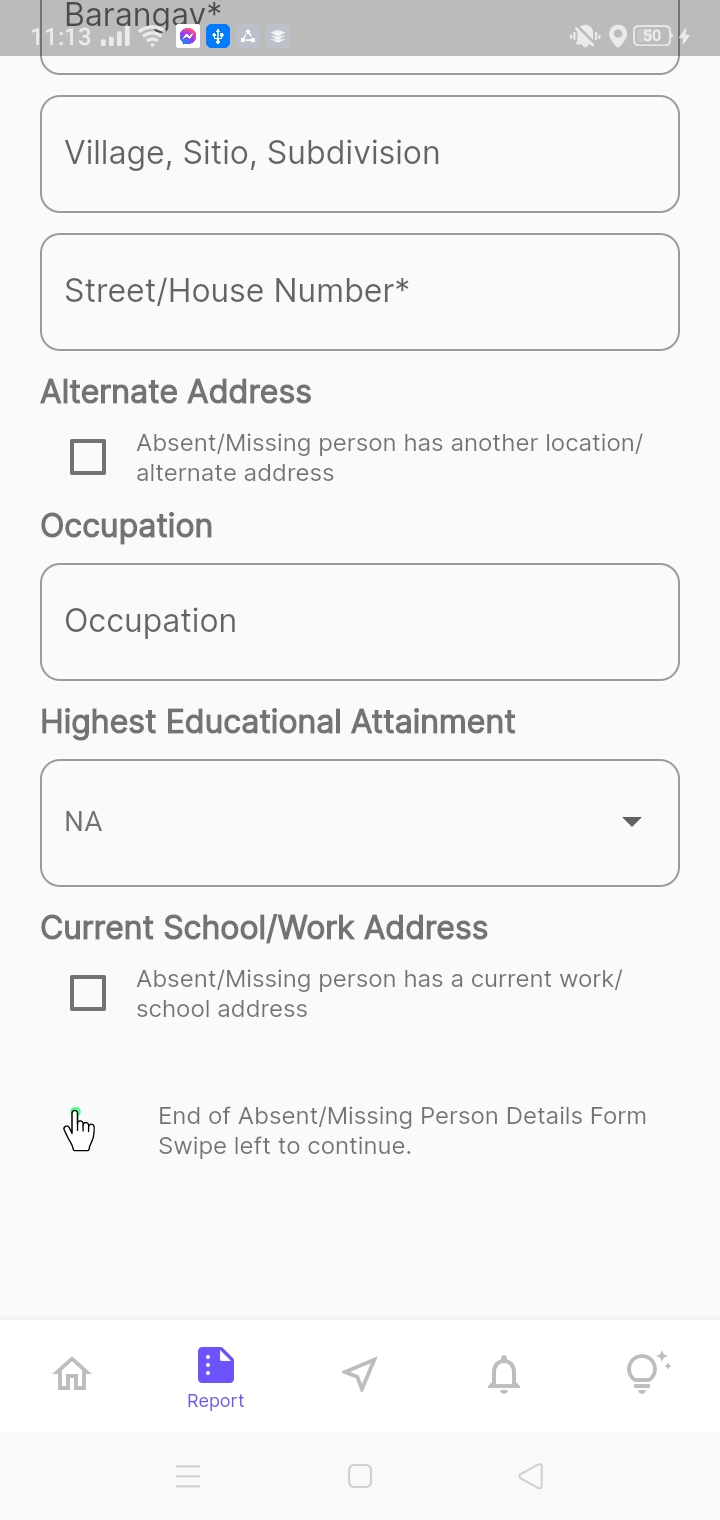
\includegraphics[scale=0.15]{figures/Chapter4/Main/p3-4.jpg}
    \end{subfigure}
    \centering
    \begin{subfigure}[c]{0.30\linewidth}
        \centering
        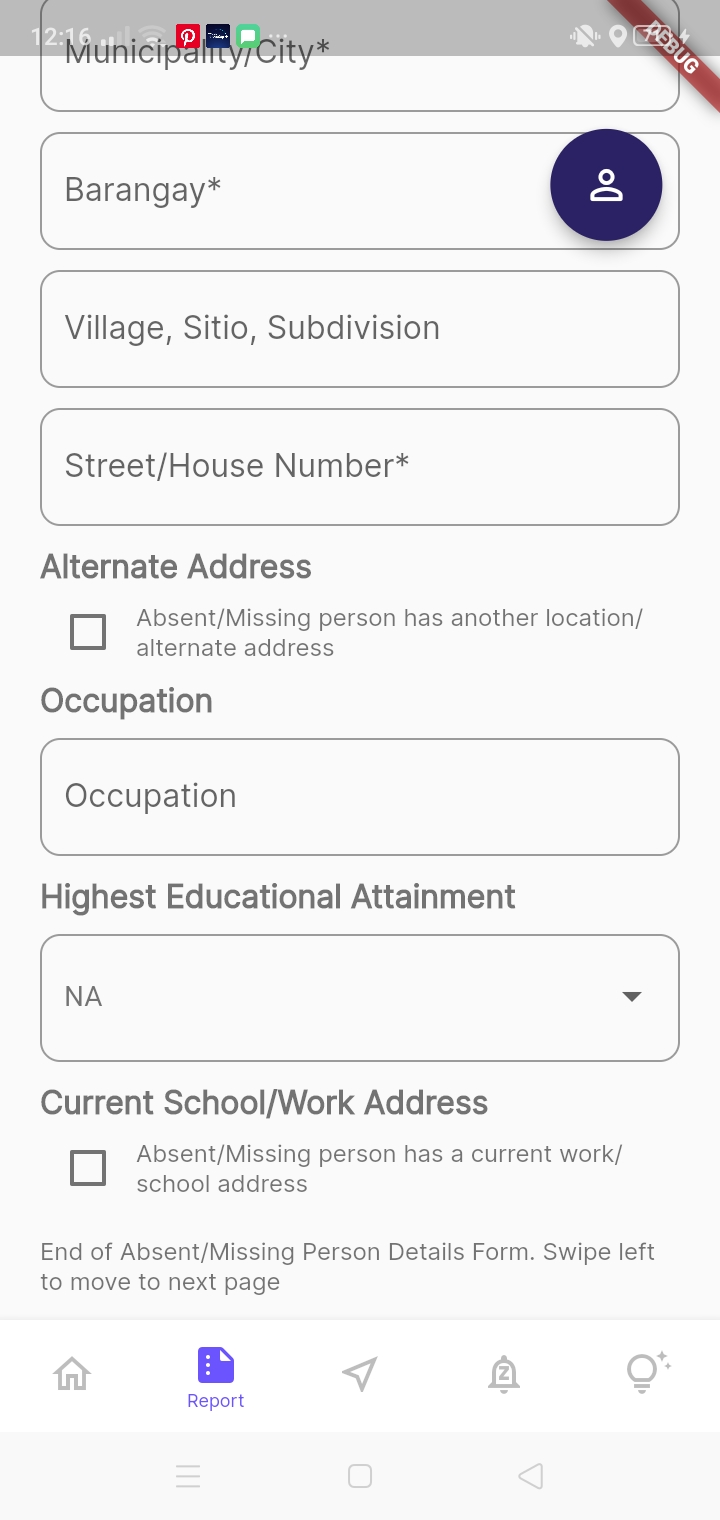
\includegraphics[scale=0.15]{figures/Chapter4/Main/p3-5.jpg}
    \end{subfigure}
    \caption{Report Form Page 3}
    \label{fig:ReportPage3}
\end{figure}


\begin{figure}[!h]
    \centering
    \begin{subfigure}[c]{0.40\linewidth}
        \centering
        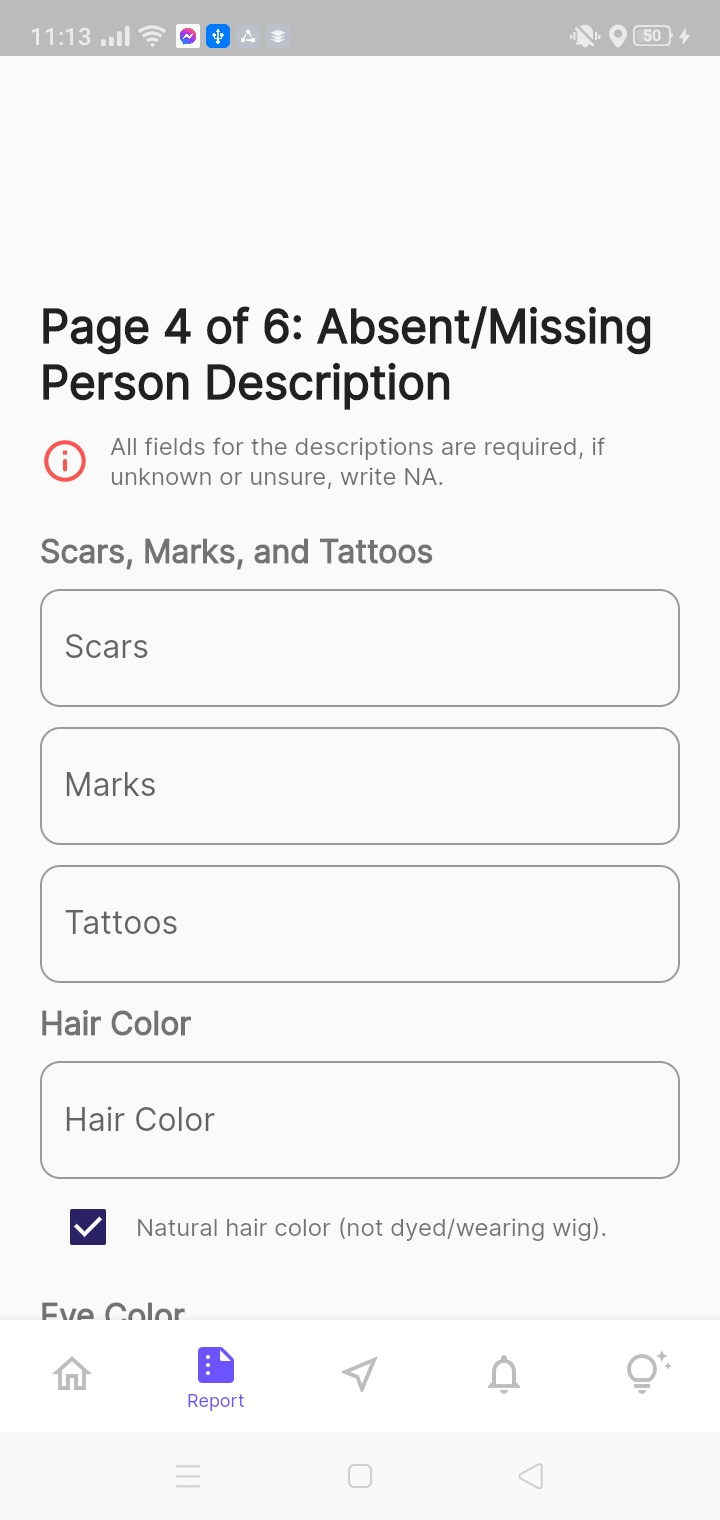
\includegraphics[scale=0.15]{figures/Chapter4/Main/p4-1.jpg}
    \end{subfigure}
    \centering
    \begin{subfigure}[c]{0.40\linewidth}
        \centering
        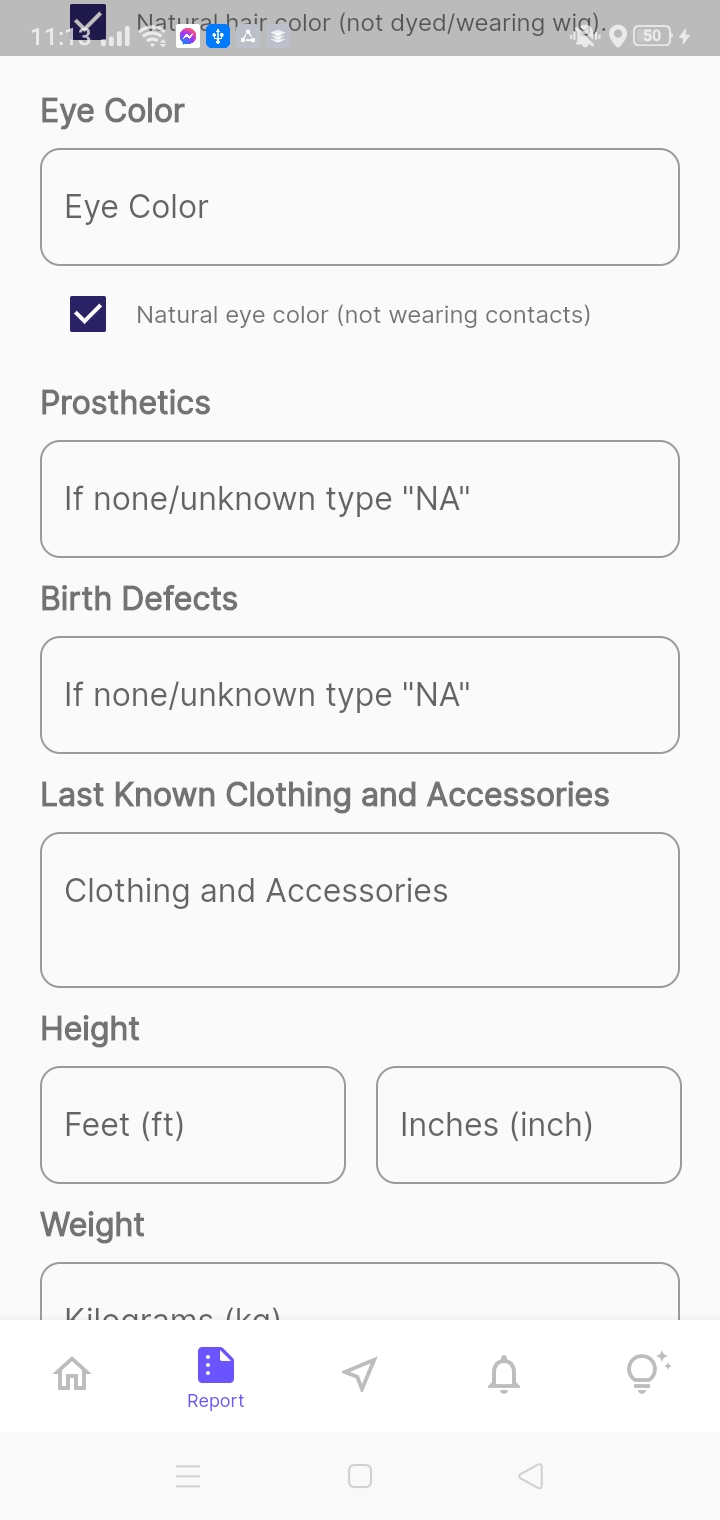
\includegraphics[scale=0.15]{figures/Chapter4/Main/p4-2.jpg}
    \end{subfigure}
    \centering
    \begin{subfigure}[c]{0.40\linewidth}
        \centering
        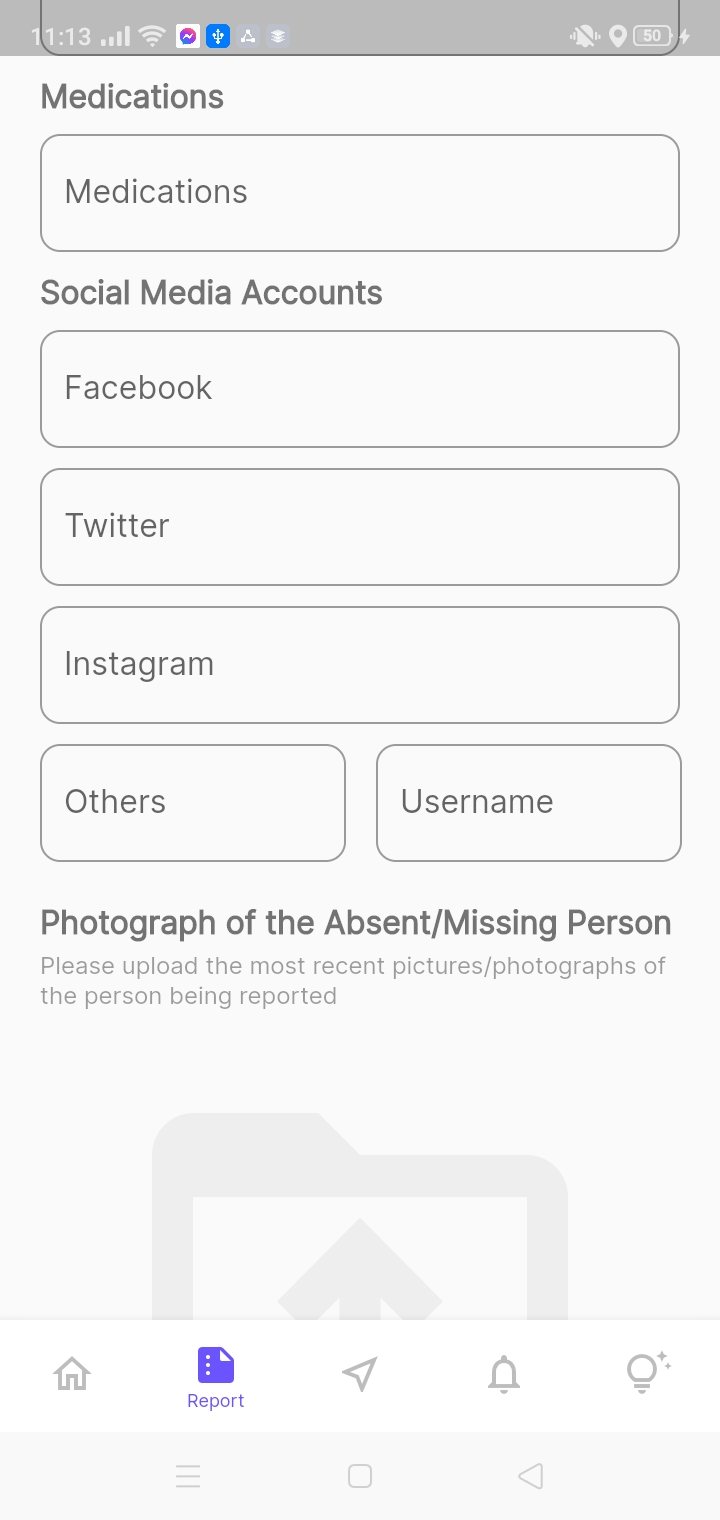
\includegraphics[scale=0.15]{figures/Chapter4/Main/p4-3.jpg}
    \end{subfigure}
        \centering
    \begin{subfigure}[c]{0.40\linewidth}
        \centering
        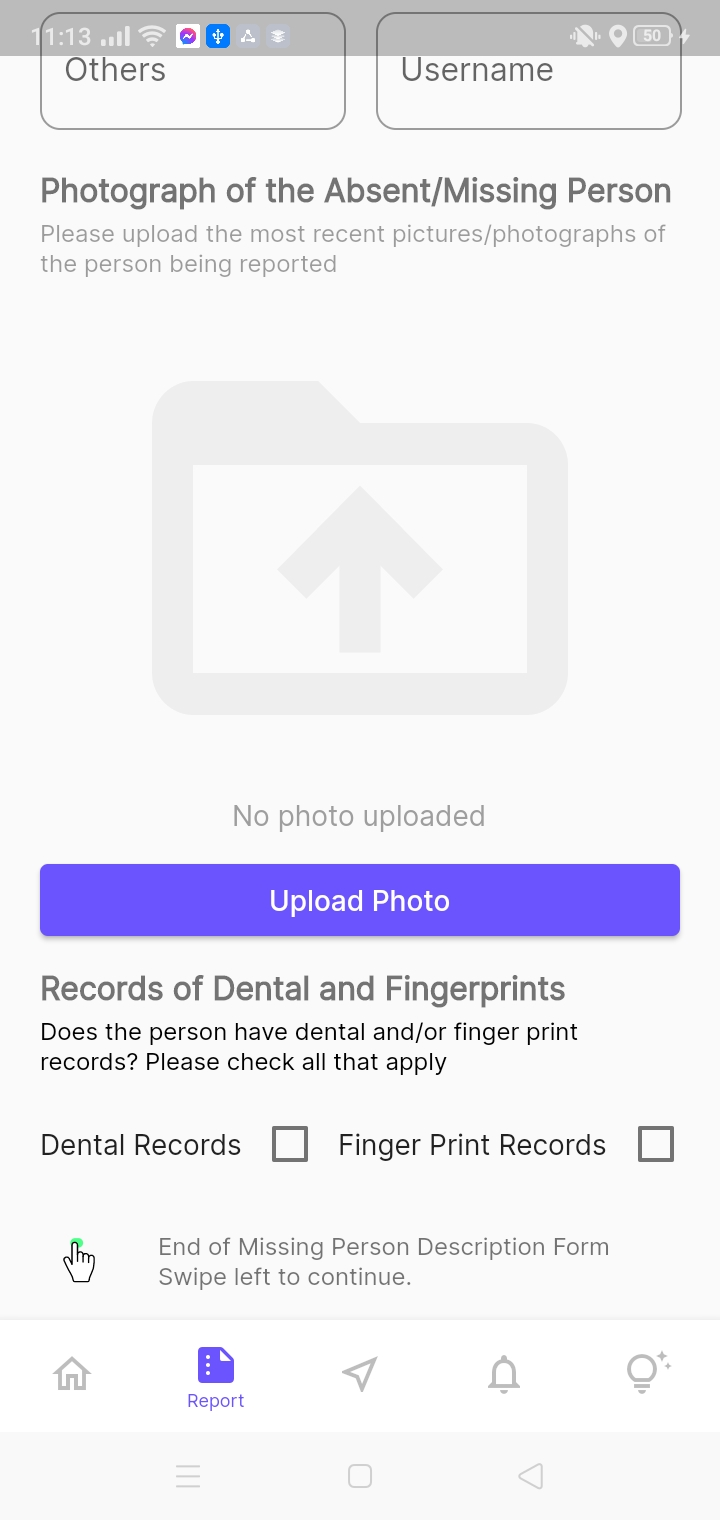
\includegraphics[scale=0.15]{figures/Chapter4/Main/p4-4.jpg}
    \end{subfigure}
    \caption{Report Form Page 4}
    \label{fig:ReportPage4}
\end{figure}
\subsubsection{Report Page 4: Absent/Missing Person Description}

The fourth page of the reports section, seen in figure \ref{fig:ReportPage4} still focuses on the information regarding the missing person. This time, however, are information relating to things that can most likely help strangers identify the missing person such as scars, marks, tattoos, hair color, eye color, prosthetic, birth defects, last known clothing and accessories, height, weight, blood type, medications, social media accounts, and of course, the last photograph of the missing person. Dental and Fingerprint records can also be added if the reportee wants to.


\begin{figure}[!h]
    \centering
    \begin{subfigure}[c]{0.30\linewidth}
        \centering
        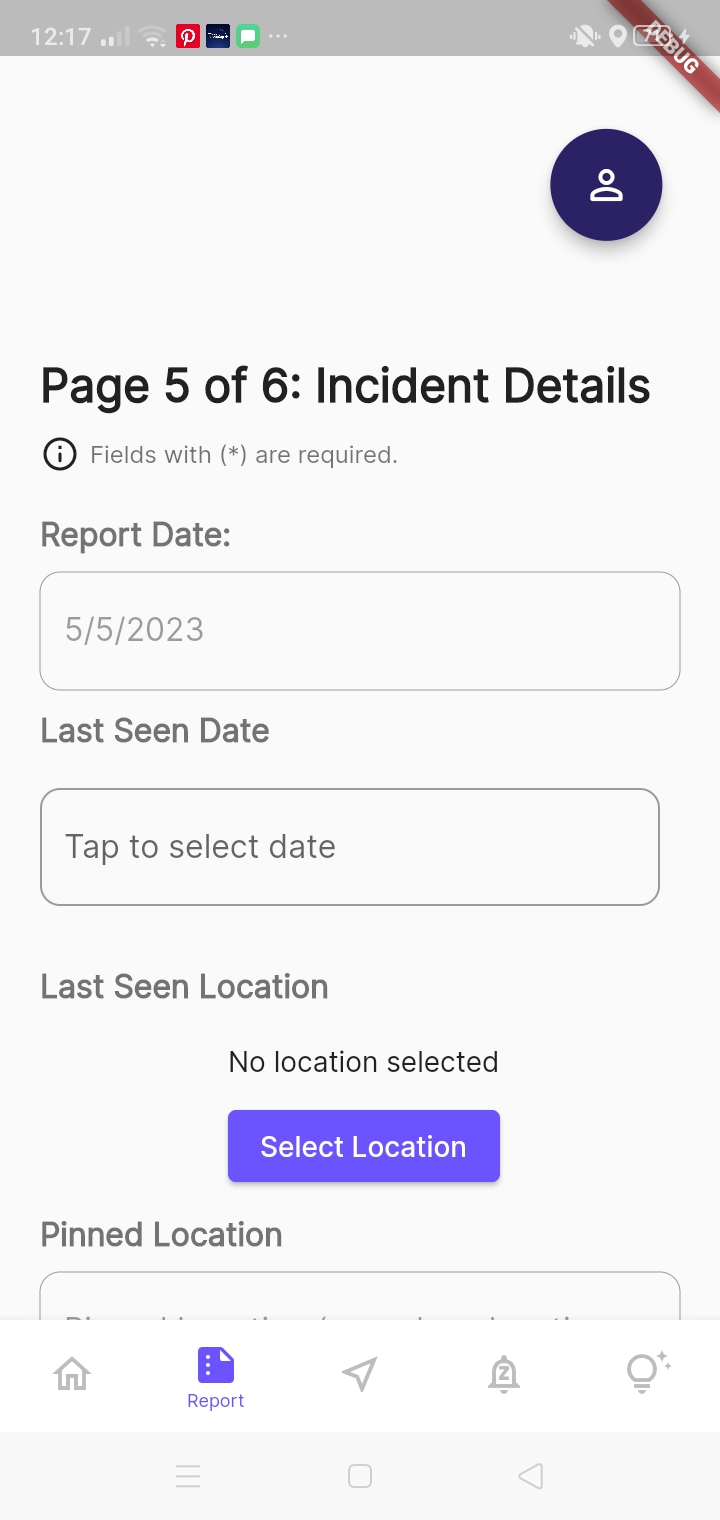
\includegraphics[scale=0.15]{figures/Chapter4/Main/p5-1.jpg}
    \end{subfigure}
    \centering
    \begin{subfigure}[c]{0.30\linewidth}
        \centering
        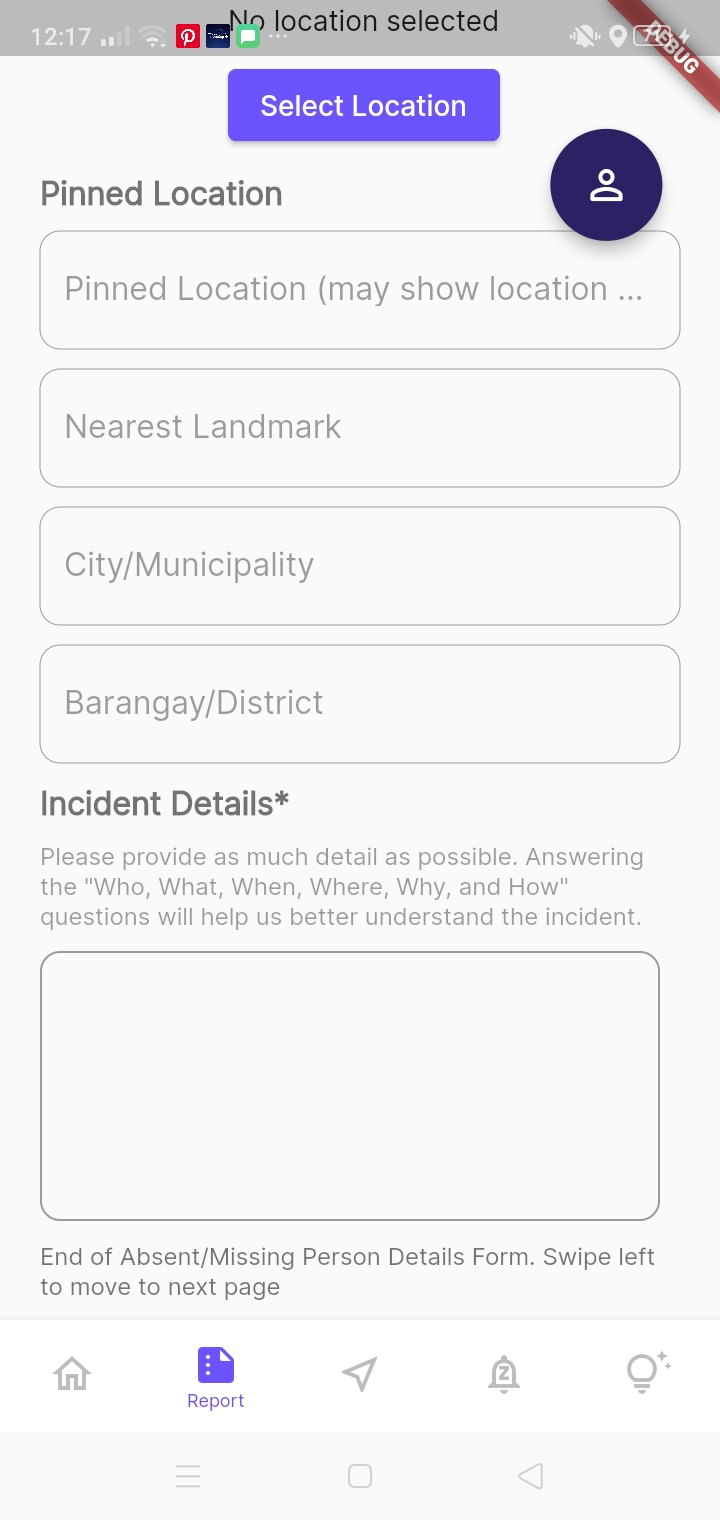
\includegraphics[scale=0.15]{figures/Chapter4/Main/p5-2.jpg}
    \end{subfigure}
    \centering
    \begin{subfigure}[c]{0.30\linewidth}
        \centering
        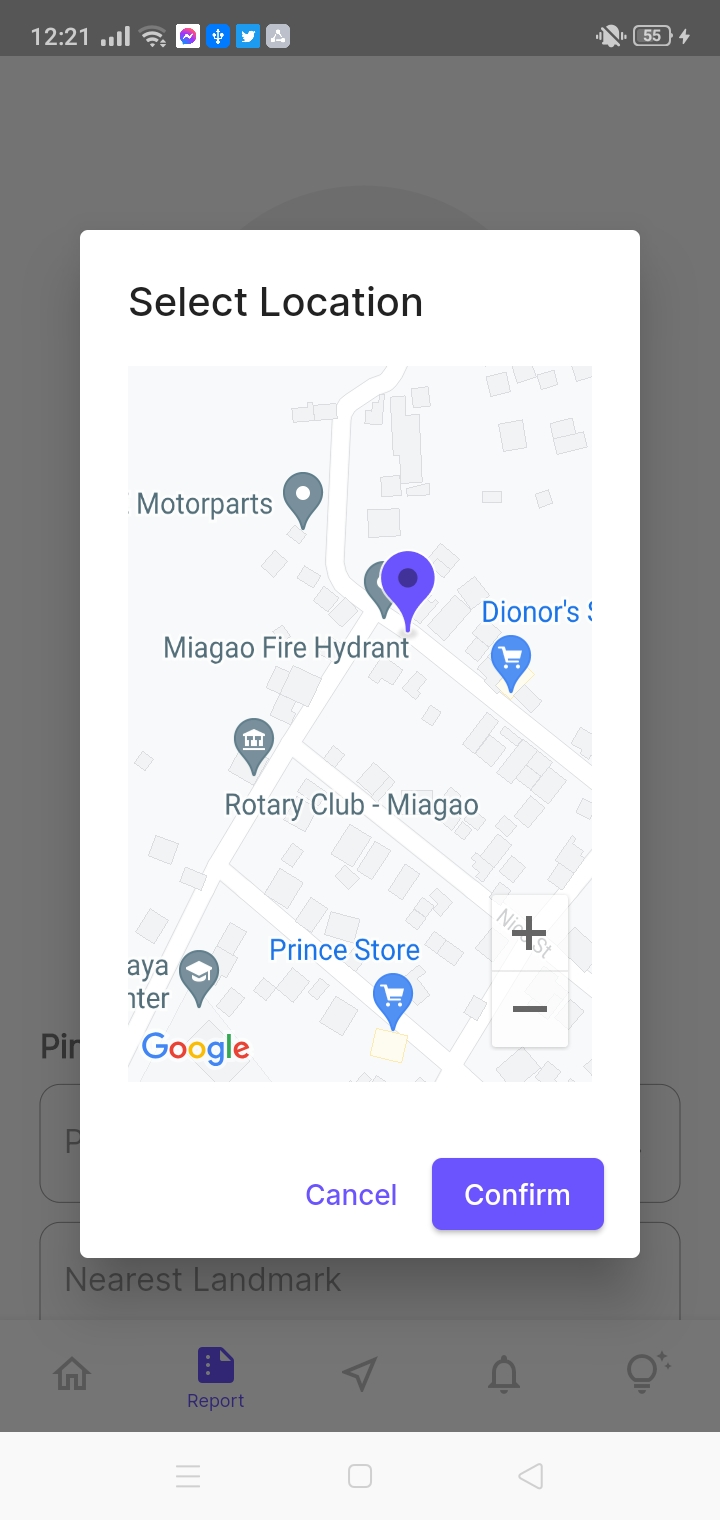
\includegraphics[scale=0.15]{figures/Chapter4/Main/p5-3.jpg}
    \end{subfigure}
    \caption{Report Form Page 5}
    \label{fig:ReportPage5}
\end{figure}
\subsubsection{Report Page 5: Incident Details}

The fifth page of the reports, as seen in figure \ref{fig:ReportPage5} requires information about the incident relating the disappearance of the missing person and is based on the "Narrative of the Incident" section of the PNP's Incident Report Form which is used for reporting incidents including those of missing persons cases.

The page requires information such as the report date, which is filled in as the current date, the last seen date, where users will be asked to select the date in a calendar when the missing person was last seen, the last seen location, where the users will be prompted to pin the location the missing person was last seen in a dialog that displays a map centered at the current location of the reportee, and the incident details, where users can input further details they deem as necessary in order to aide in the finding of the missing person. 

\begin{figure}[!h]
    \centering
    \begin{subfigure}[c]{0.40\linewidth}
        \centering
        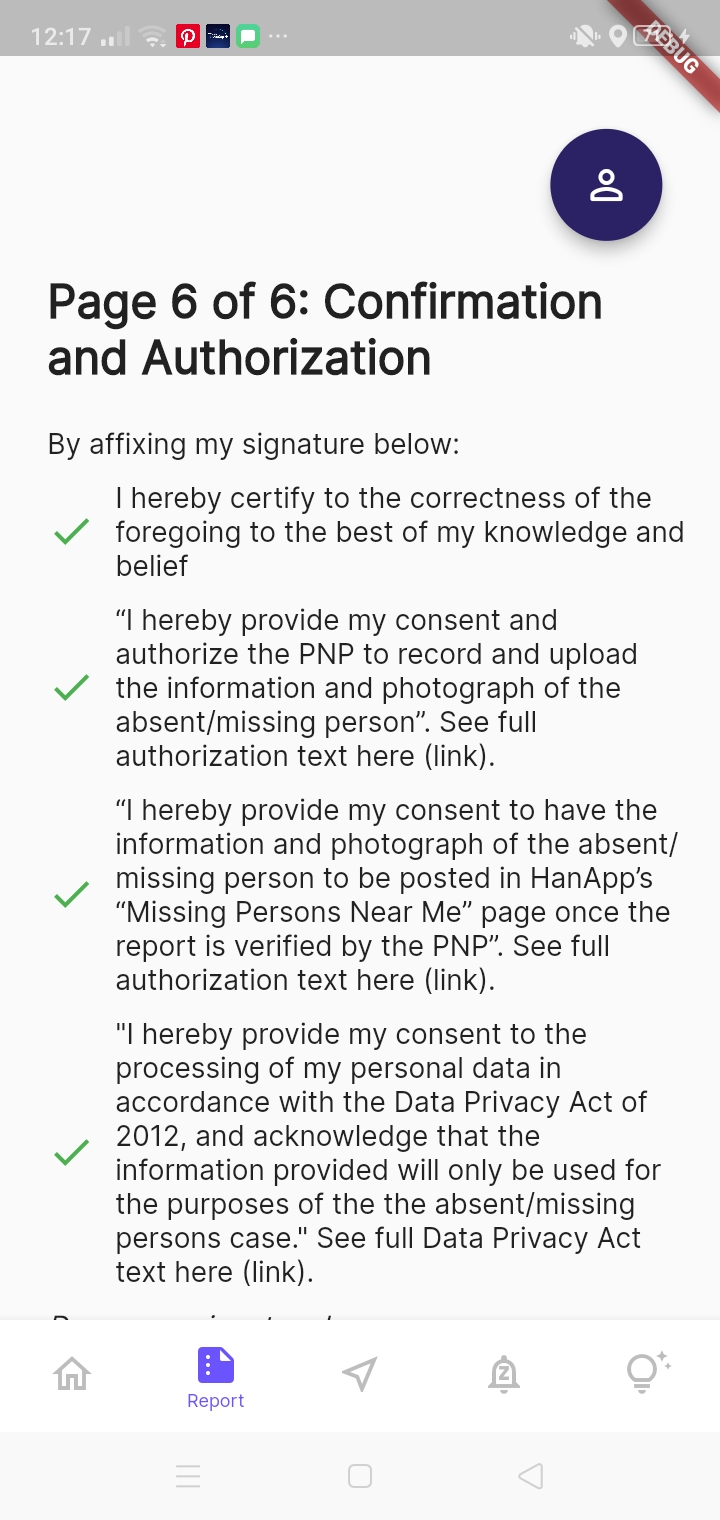
\includegraphics[scale=0.15]{figures/Chapter4/Main/p6-1.jpg}
    \end{subfigure}
    \centering
    \begin{subfigure}[c]{0.40\linewidth}
        \centering
        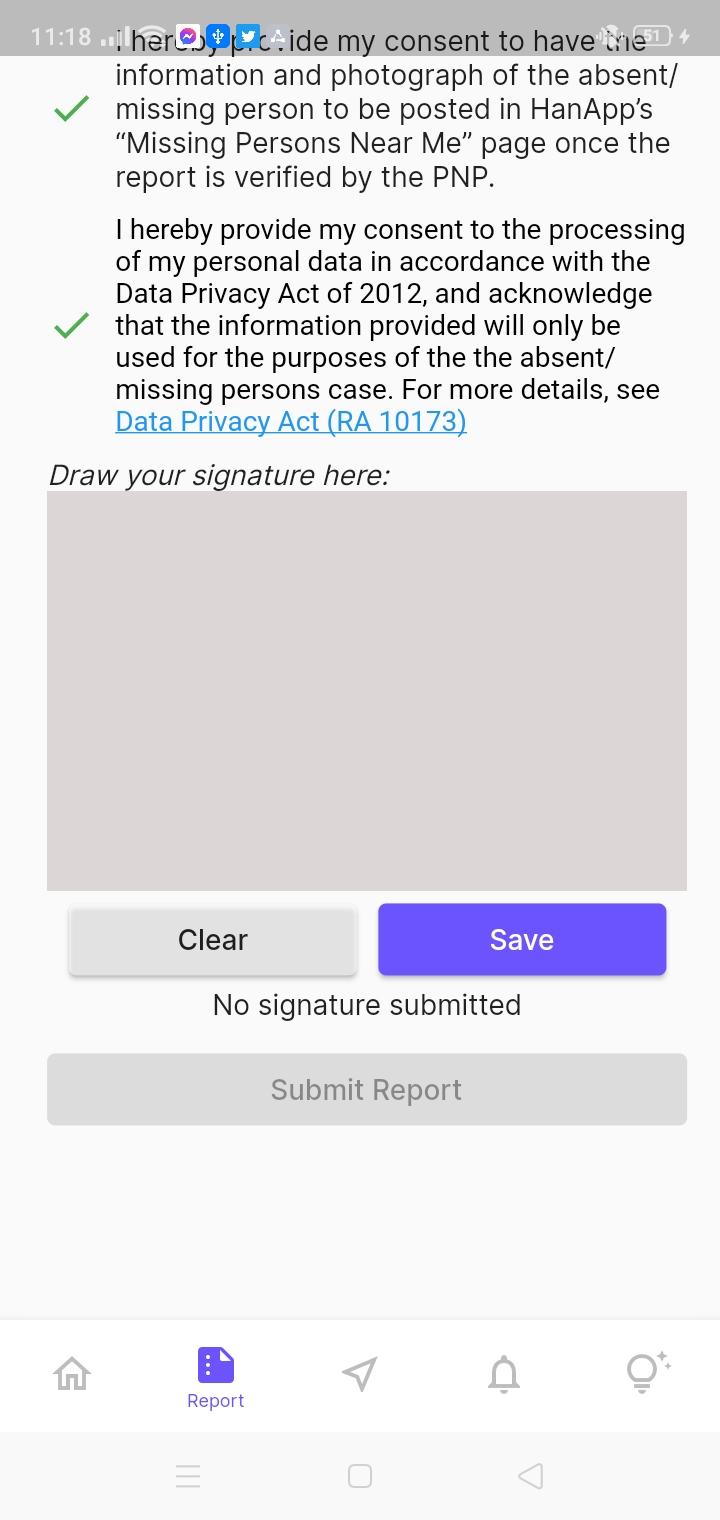
\includegraphics[scale=0.15]{figures/Chapter4/Main/p6-2.jpg}
    \end{subfigure}
    \caption{Report Form Page 6}
    \label{fig:ReportPage6}
\end{figure}
\subsubsection{Report Page 6: Confirmation and Authorization}

The sixth, and the last page, as seen in figure \ref{fig:ReportPage6} asks for the confirmation and authorization of the user to finally submit the report that they have filled out. The page would require the signature of the reportee on the signature pad provided citing that, by signing the report, they agree to have the information submitted published and adhere to the rules and responsibilities that come with them submitting the report to the PNP interface for verification. After which, the users can then submit the form to PNP.

\subsection{Nearby Page}

\begin{figure}[!h]
    \centering
    \begin{subfigure}[c]{0.30\linewidth}
        \centering
        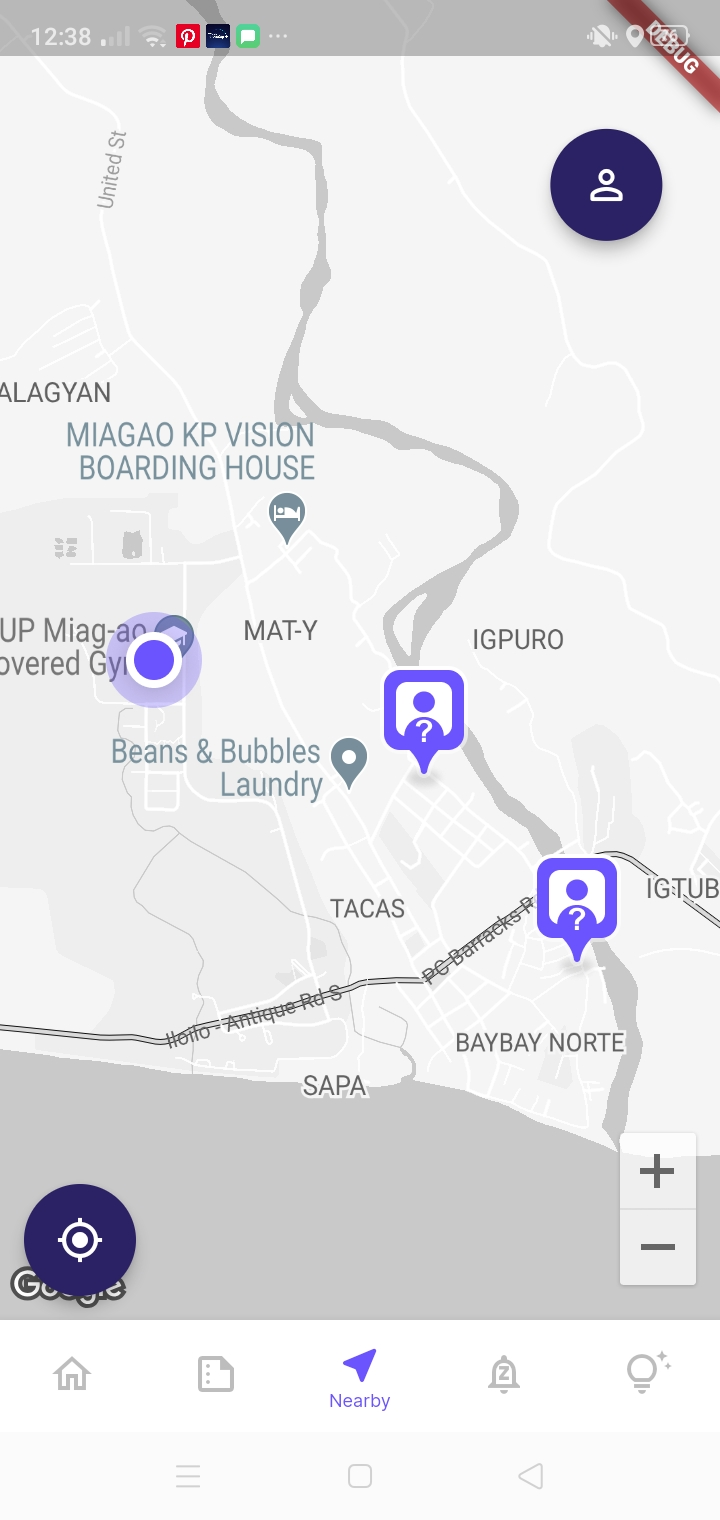
\includegraphics[scale=0.15]{figures/Chapter4/Main/Nearby-3.jpg}
    \end{subfigure}
    \centering
    \begin{subfigure}[c]{0.30\linewidth}
        \centering
        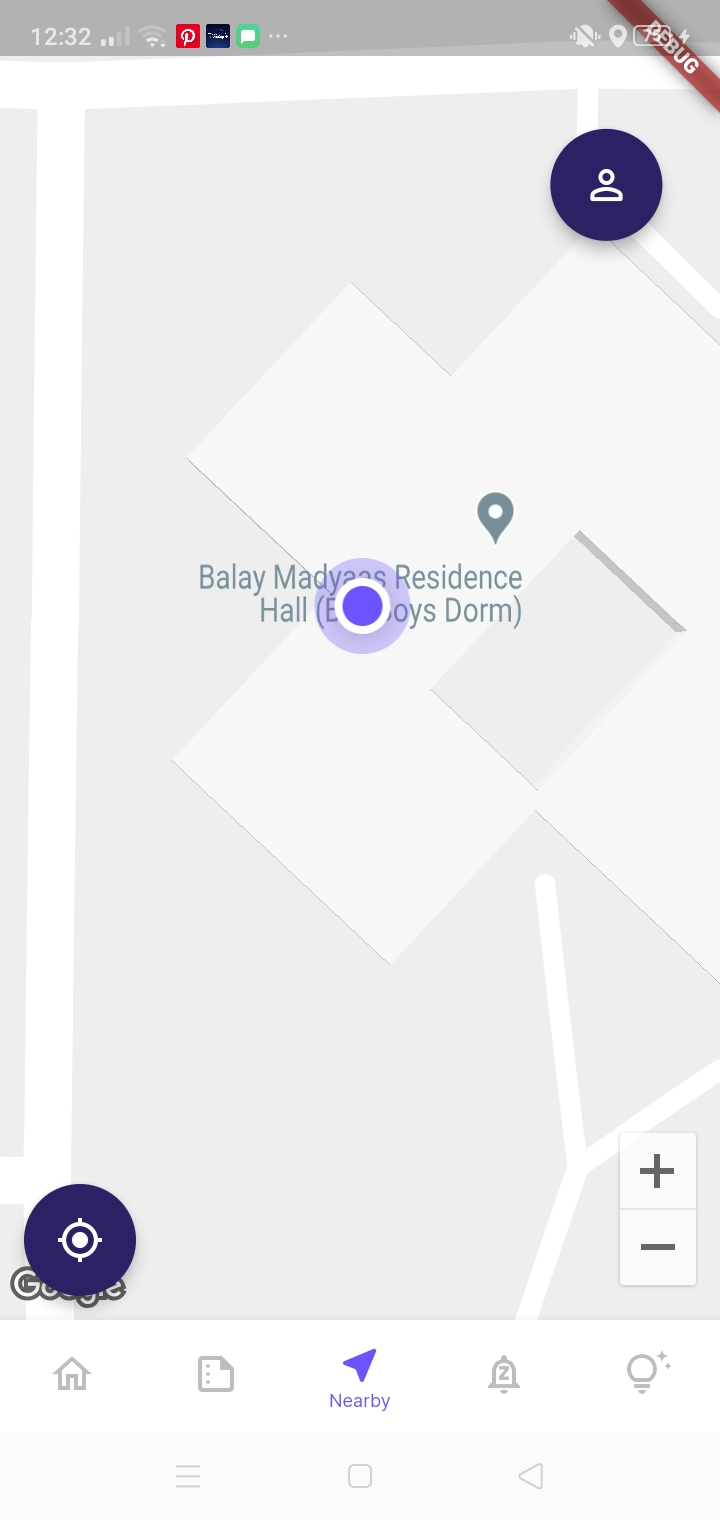
\includegraphics[scale=0.15]{figures/Chapter4/Main/Nearby-2.jpg}
    \end{subfigure}
    \caption{Missing Persons and User Location in Nearby}
    \label{fig:userTracking}
\end{figure}
Figure \ref{fig:userTracking} is the interface of tracking missing persons near the user. A location marker will guide the current or last seen whereabouts of a missing person. Only the verified reports that was identified by the PNP through their reports management suite will only be shown. This will allow reports to be validated thoroughly on their end. Apart from that, the user has the liberty to navigate the map, may it be street view or city-wide view by pinching the screen. Also, users can zoom in and zoom out depending on their preference. Landmarks and familiar streets will be shown to guide the users easily on the whereabouts of the missing person. Considering, for example, that a 5-km radius will be visible, it will then encircle the last place the MP was seen. Another thing that the application also wants to note is how the user can tap on the MPs icon to see the details of descriptions pertaining to the individual. Importantly, there is an additional feature that permits the user to find the nearest route going to the last seen location of the missing person by clicking the 'right turn' icon that will redirect them to Google Maps app, given that they have it on their phone installed. Through all of this, it will enable a swift identification of the person and give the authorities a leeway to make necessary course of action to find these reported missing persons.

\subsection{Updates Page}

Figure \ref{fig:userReportStatus} demonstrates how the user can visibly see the status of their reported missing persons through the Updates section. For instance, when the user submits their report, the PNP has the liberty to change the status of their report given the information that was forwarded to them as shown in Figure \ref{fig:PNP2}. Not only that, but they will also inspect and verify these as it is sensitive and crucial at this point to confirm whether it needs urgent attention or not (reports with incomplete details would be a factor here). The update of the status is real-time, so when the PNP change its status to a different one, it will automatically change in the user side. The update tags of the reports will consist of four (4) statuses to choose from, namely, Received, Verified, Rejected, or Found. All of these are directly shown to the Updates section of the user's account.

\begin{figure}[!h]
    \centering
    \begin{subfigure}[c]{0.20\linewidth}
        \centering
        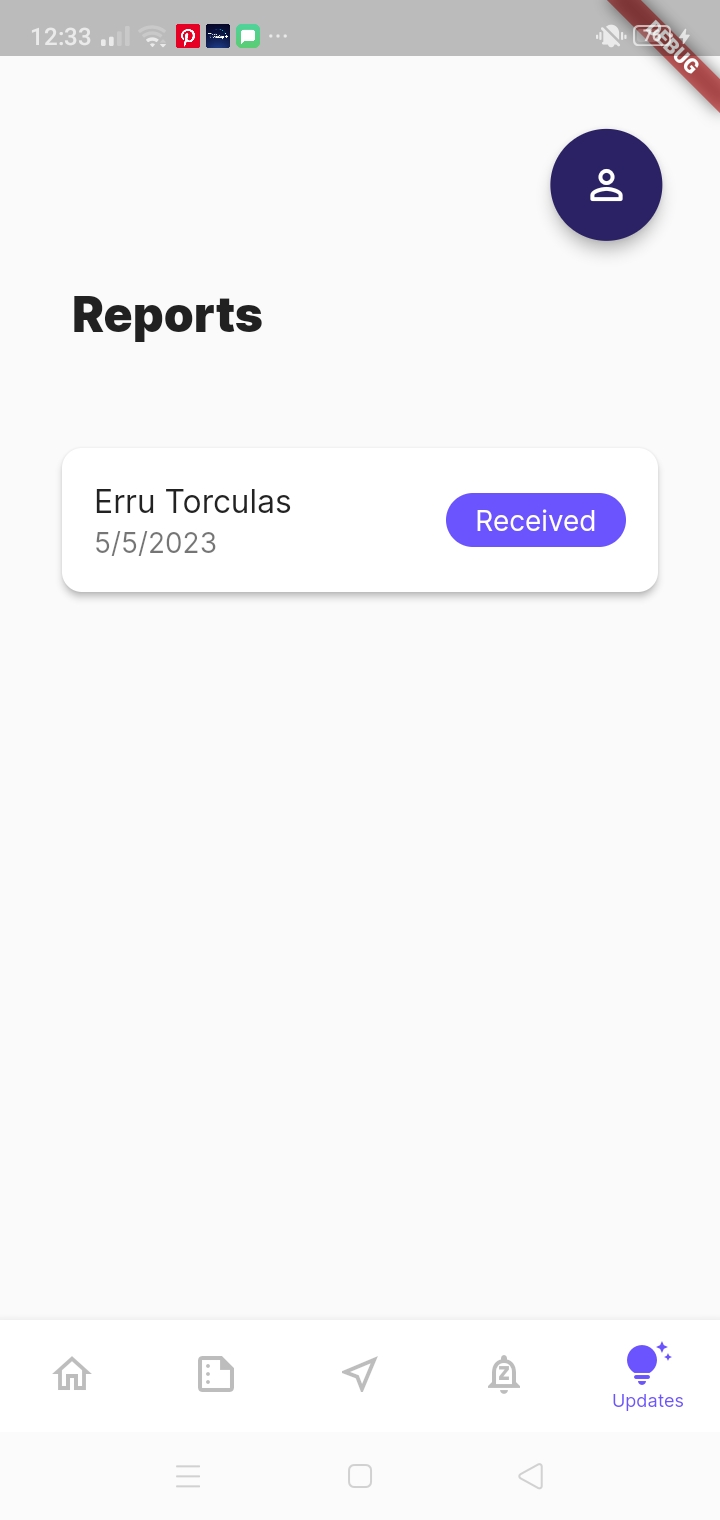
\includegraphics[scale=0.10]{figures/Chapter4/Main/Report-1.jpg}
        \caption{Received}
        \label{fig:StatusReceived}
    \end{subfigure}
    \centering
    \begin{subfigure}[c]{0.20\linewidth}
        \centering
        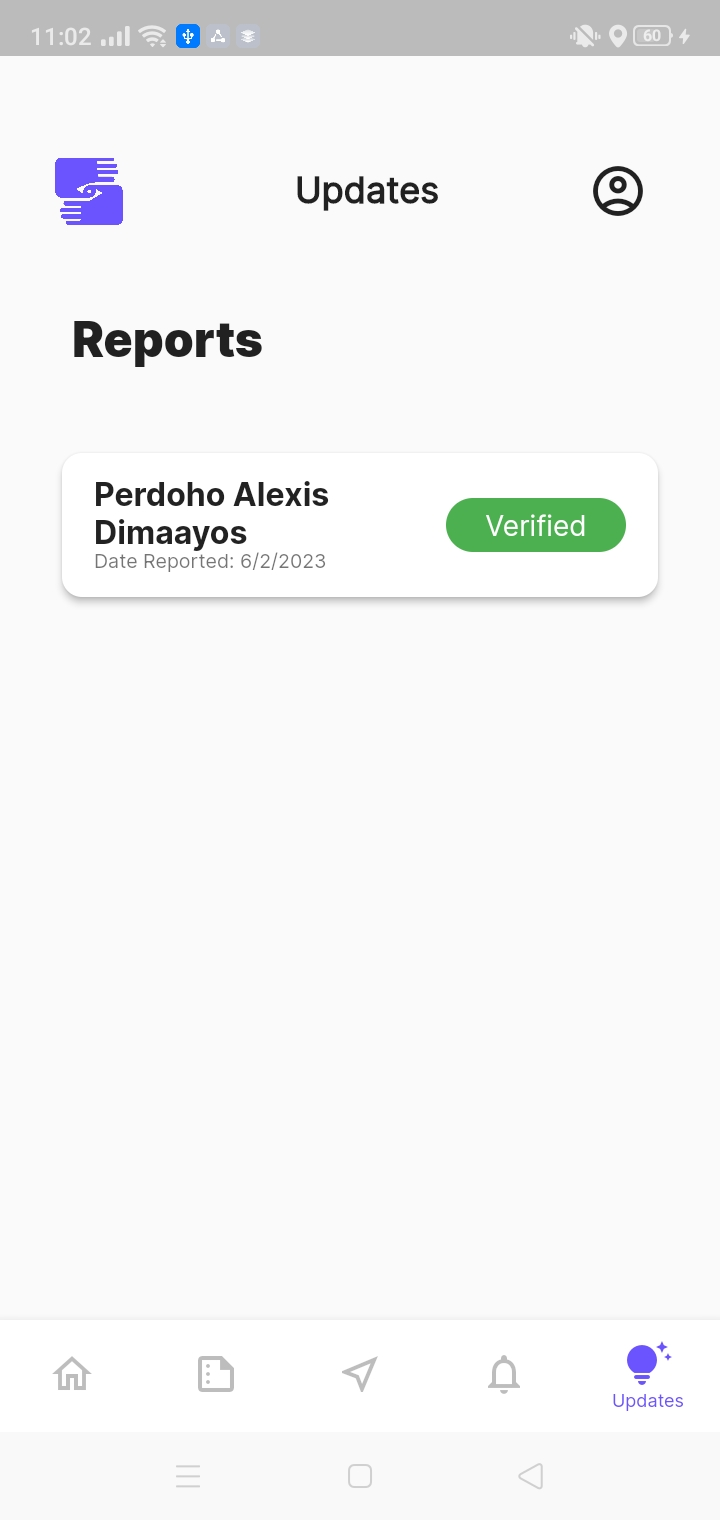
\includegraphics[scale=0.10]{figures/Chapter4/Main/Report-2.jpg}
        \caption{Verified}
        \label{fig:StatusVerified}
    \end{subfigure}
    \centering
    \begin{subfigure}[c]{0.20\linewidth}
        \centering
        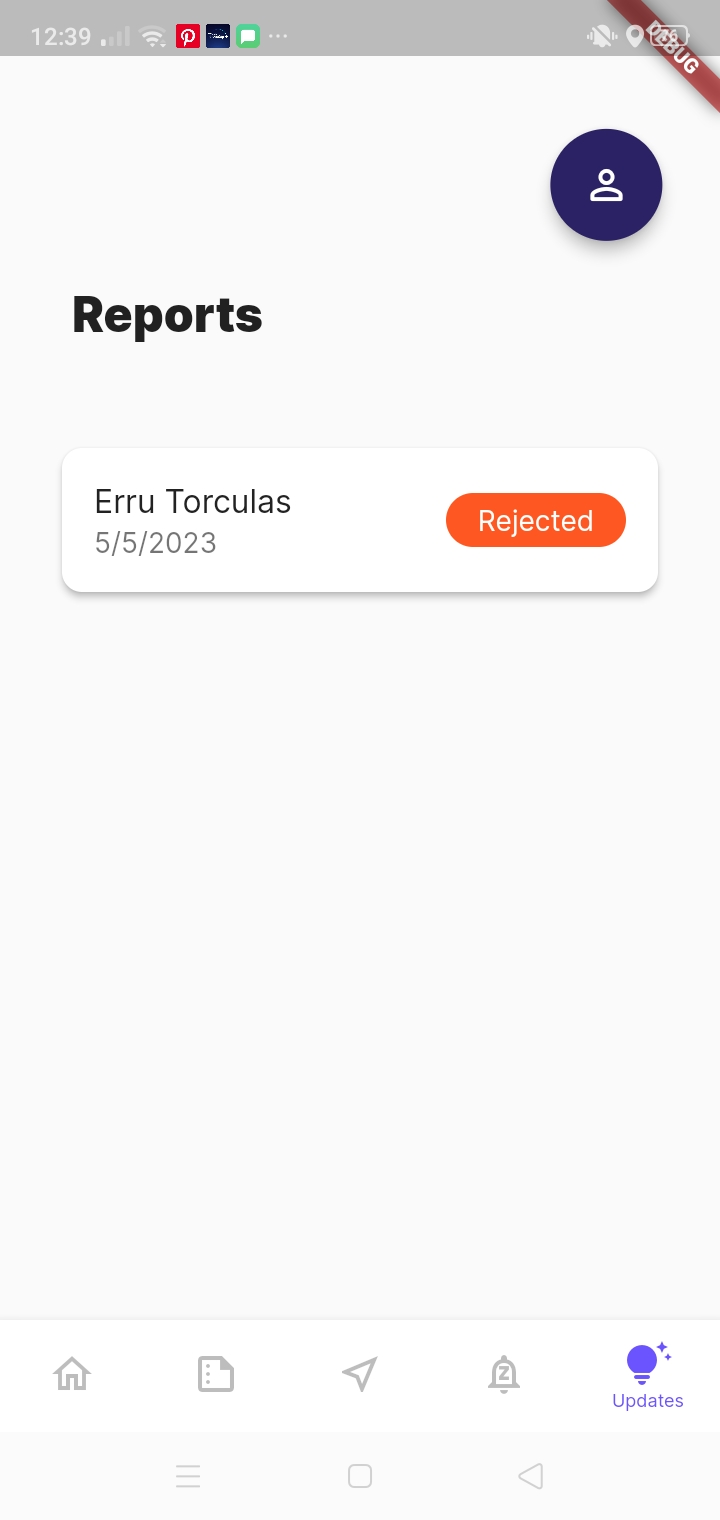
\includegraphics[scale=0.10]{figures/Chapter4/Main/Report-3.jpg}
        \caption{Rejected}
        \label{fig:StatusRejected}
    \end{subfigure}
        \centering
    \begin{subfigure}[c]{0.20\linewidth}
        \centering
        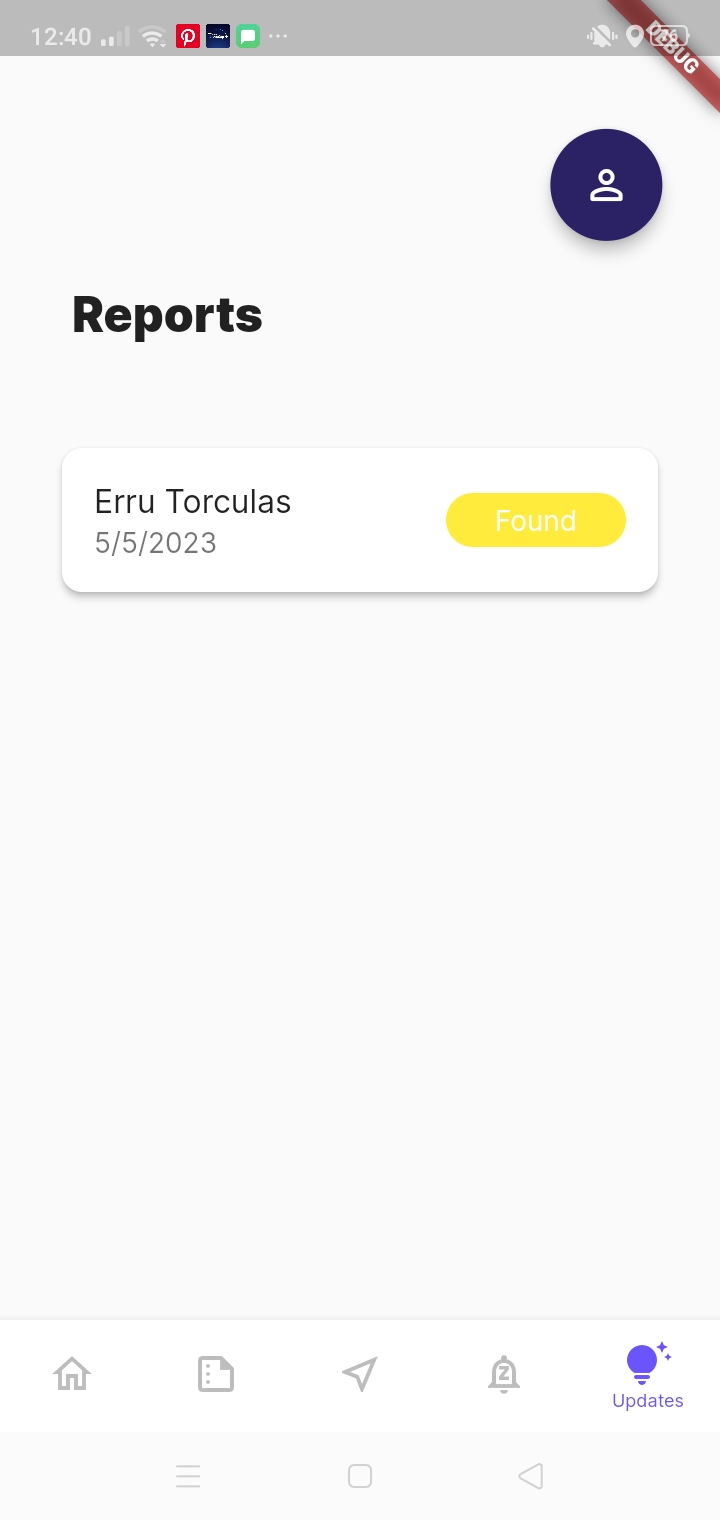
\includegraphics[scale=0.10]{figures/Chapter4/Main/Report-4.jpg}
        \caption{Found}
        \label{fig:StatusFound}
    \end{subfigure}
    \caption{Updates Page with Status of Report}
    \label{fig:userReportStatus}
\end{figure}

\section{UI/UX Design Implementation}

\subsection{Application Suite Logo}

The HanApp logo, as seen in Figure \ref{fig:hanappLogo}, is an indigo-colored logo of two horizontally-oriented hands whose thumbs meet in between and form an "eye", and with the fingers forming "speed lines". The two hands in the logo have various meanings: (1) connecting the PNP and the reporter, (2) connecting the reporter to the general community, and (3) the missing person reuniting with the reporter, whereas the eye in the middle imply that the application is about looking for missing persons. Moreover, the "speed lines" formed by the fingers help imply that the application makes the process of reporting, verifying, disseminating, and resolving missing persons cases faster. 

As such, HanApp logo meets the application logo requirement such that it is distinct, meaningful, and cohesive with the HanApp's UI/UX design and color theme.
\begin{figure}[!h]
    \centering
    \begin{minipage}[c]{0.50\linewidth}
        \centering
        
\includegraphics[scale=0.15]{figures/hanappLogo.png}
        \caption{Report Form Page 1}
        \label{fig:hanappLogo}
    \end{minipage}
\end{figure}

\subsection{UI/UX Design}

As shown in the preceding sections, the UI/UX design of the application suite were able to meet the UI/UX Design requirements listed in the previous chapter, namely:

\begin{enumerate}
    \item The application's frontend design ensures accessibility and ease of use in its choice of font size and family, layout, and colors.
    \item The English language is utilized throughout the entire application with no grammatical errors and with the use of simple and straightforward wordings.
    \item The report form pages were simplified and incorporated the use of checkboxes, radio buttons, buttons for save/upload prompts, and text fields as well as validators, ensuring not only ease of use but also the completeness and correctness in the submitted reports. 
\end{enumerate}

\section{Backend Framework - Firebase}

Firebase handles both account management and data management. As such, the following sections will discuss and show the backend framework at which user accounts and reports data is stored and managed.

\subsection{User Accounts Authentication and Storage}

As seen in Figure \ref{fig:firebaseAuth}, user accounts are stored in Firebase's Authentication page. It shows the user account's unique UID, email, date created, and last signed in page. Firebase also handles the authentication service which was shown in the user account authentication section above.
\begin{figure}[!h]
    \centering
    \begin{minipage}[c]{1\linewidth}
        \centering
        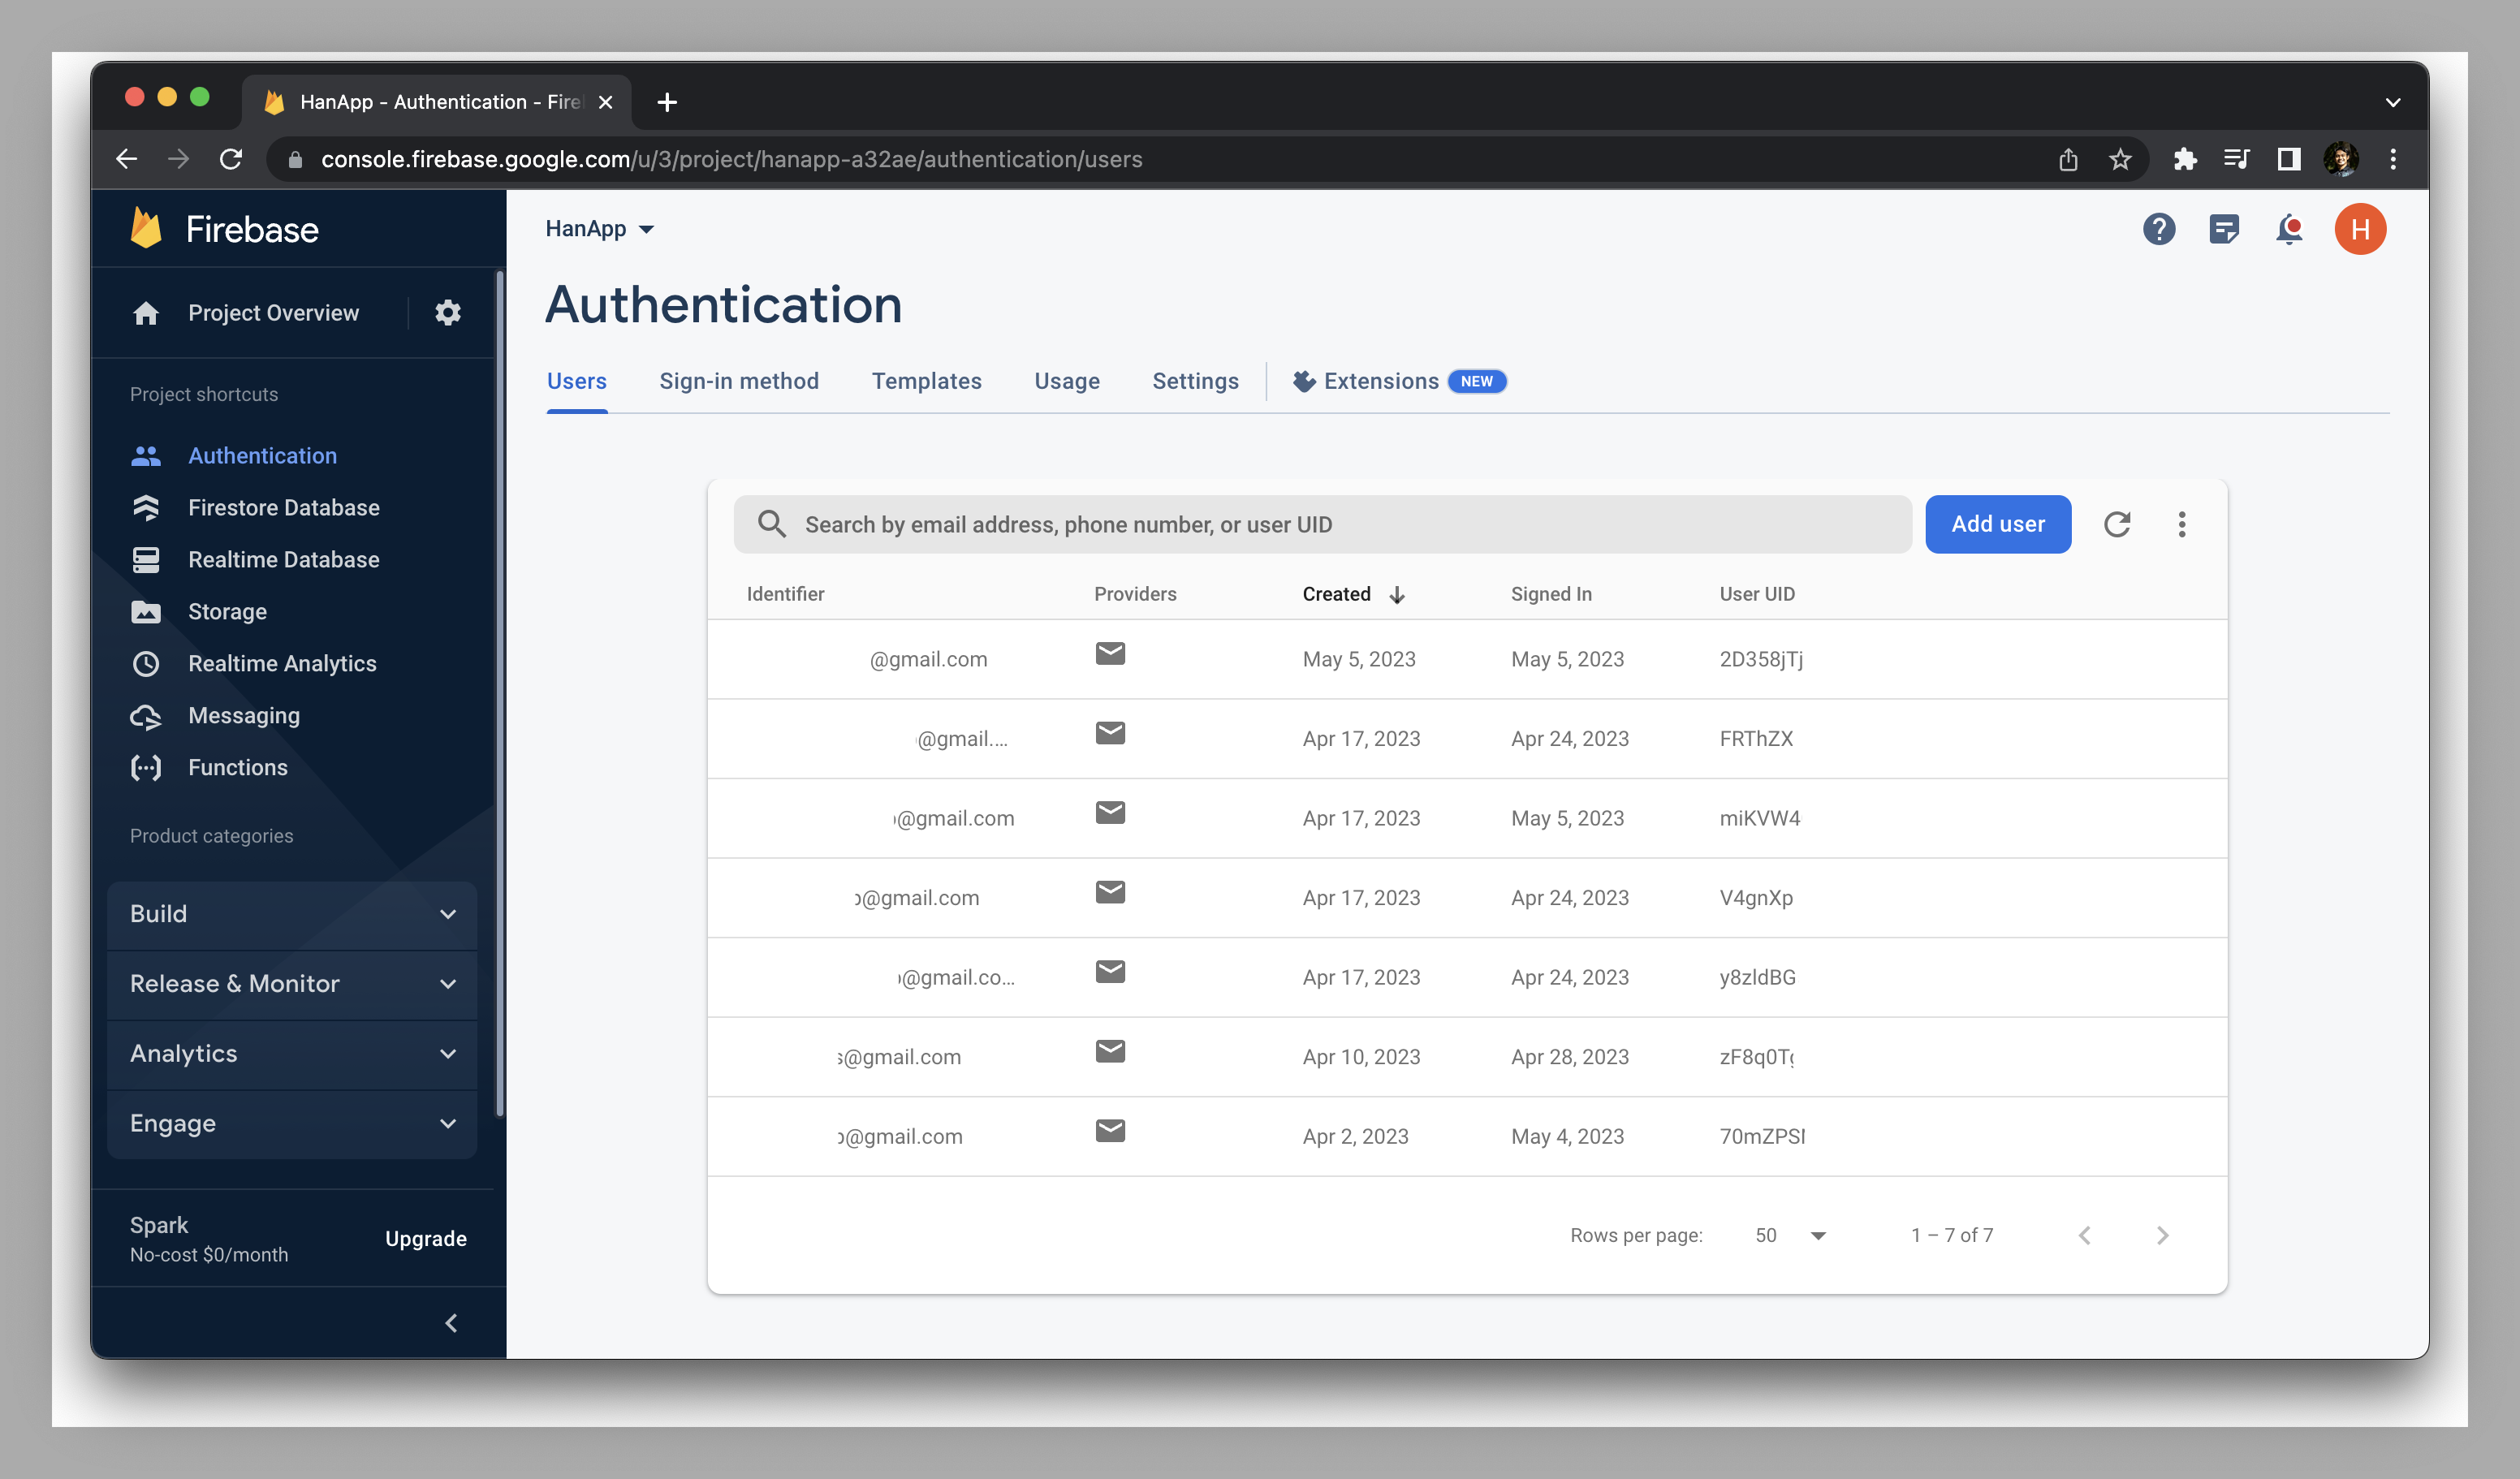
\includegraphics[scale=0.25]{figures/Chapter4/Firebase/authentication.png}
        \caption{Authentication Database}
        \label{fig:firebaseAuth}
    \end{minipage}
\end{figure}
\subsection{Realtime Database (RTDB) for User Data and Reports}

All user data (for main and PNP accounts) and their reports are stored in the RTDB as seen in Figure \ref{fig:firebaseRTDB}. There are three main "nodes" storing the Main Users user data, PNP Accounts user data, and Reports data. The Reports node stores and organizes all reports that have been submitted through the application under each user.
\begin{figure}[!h]
    \centering
    \begin{minipage}[c]{1\linewidth}
        \centering
        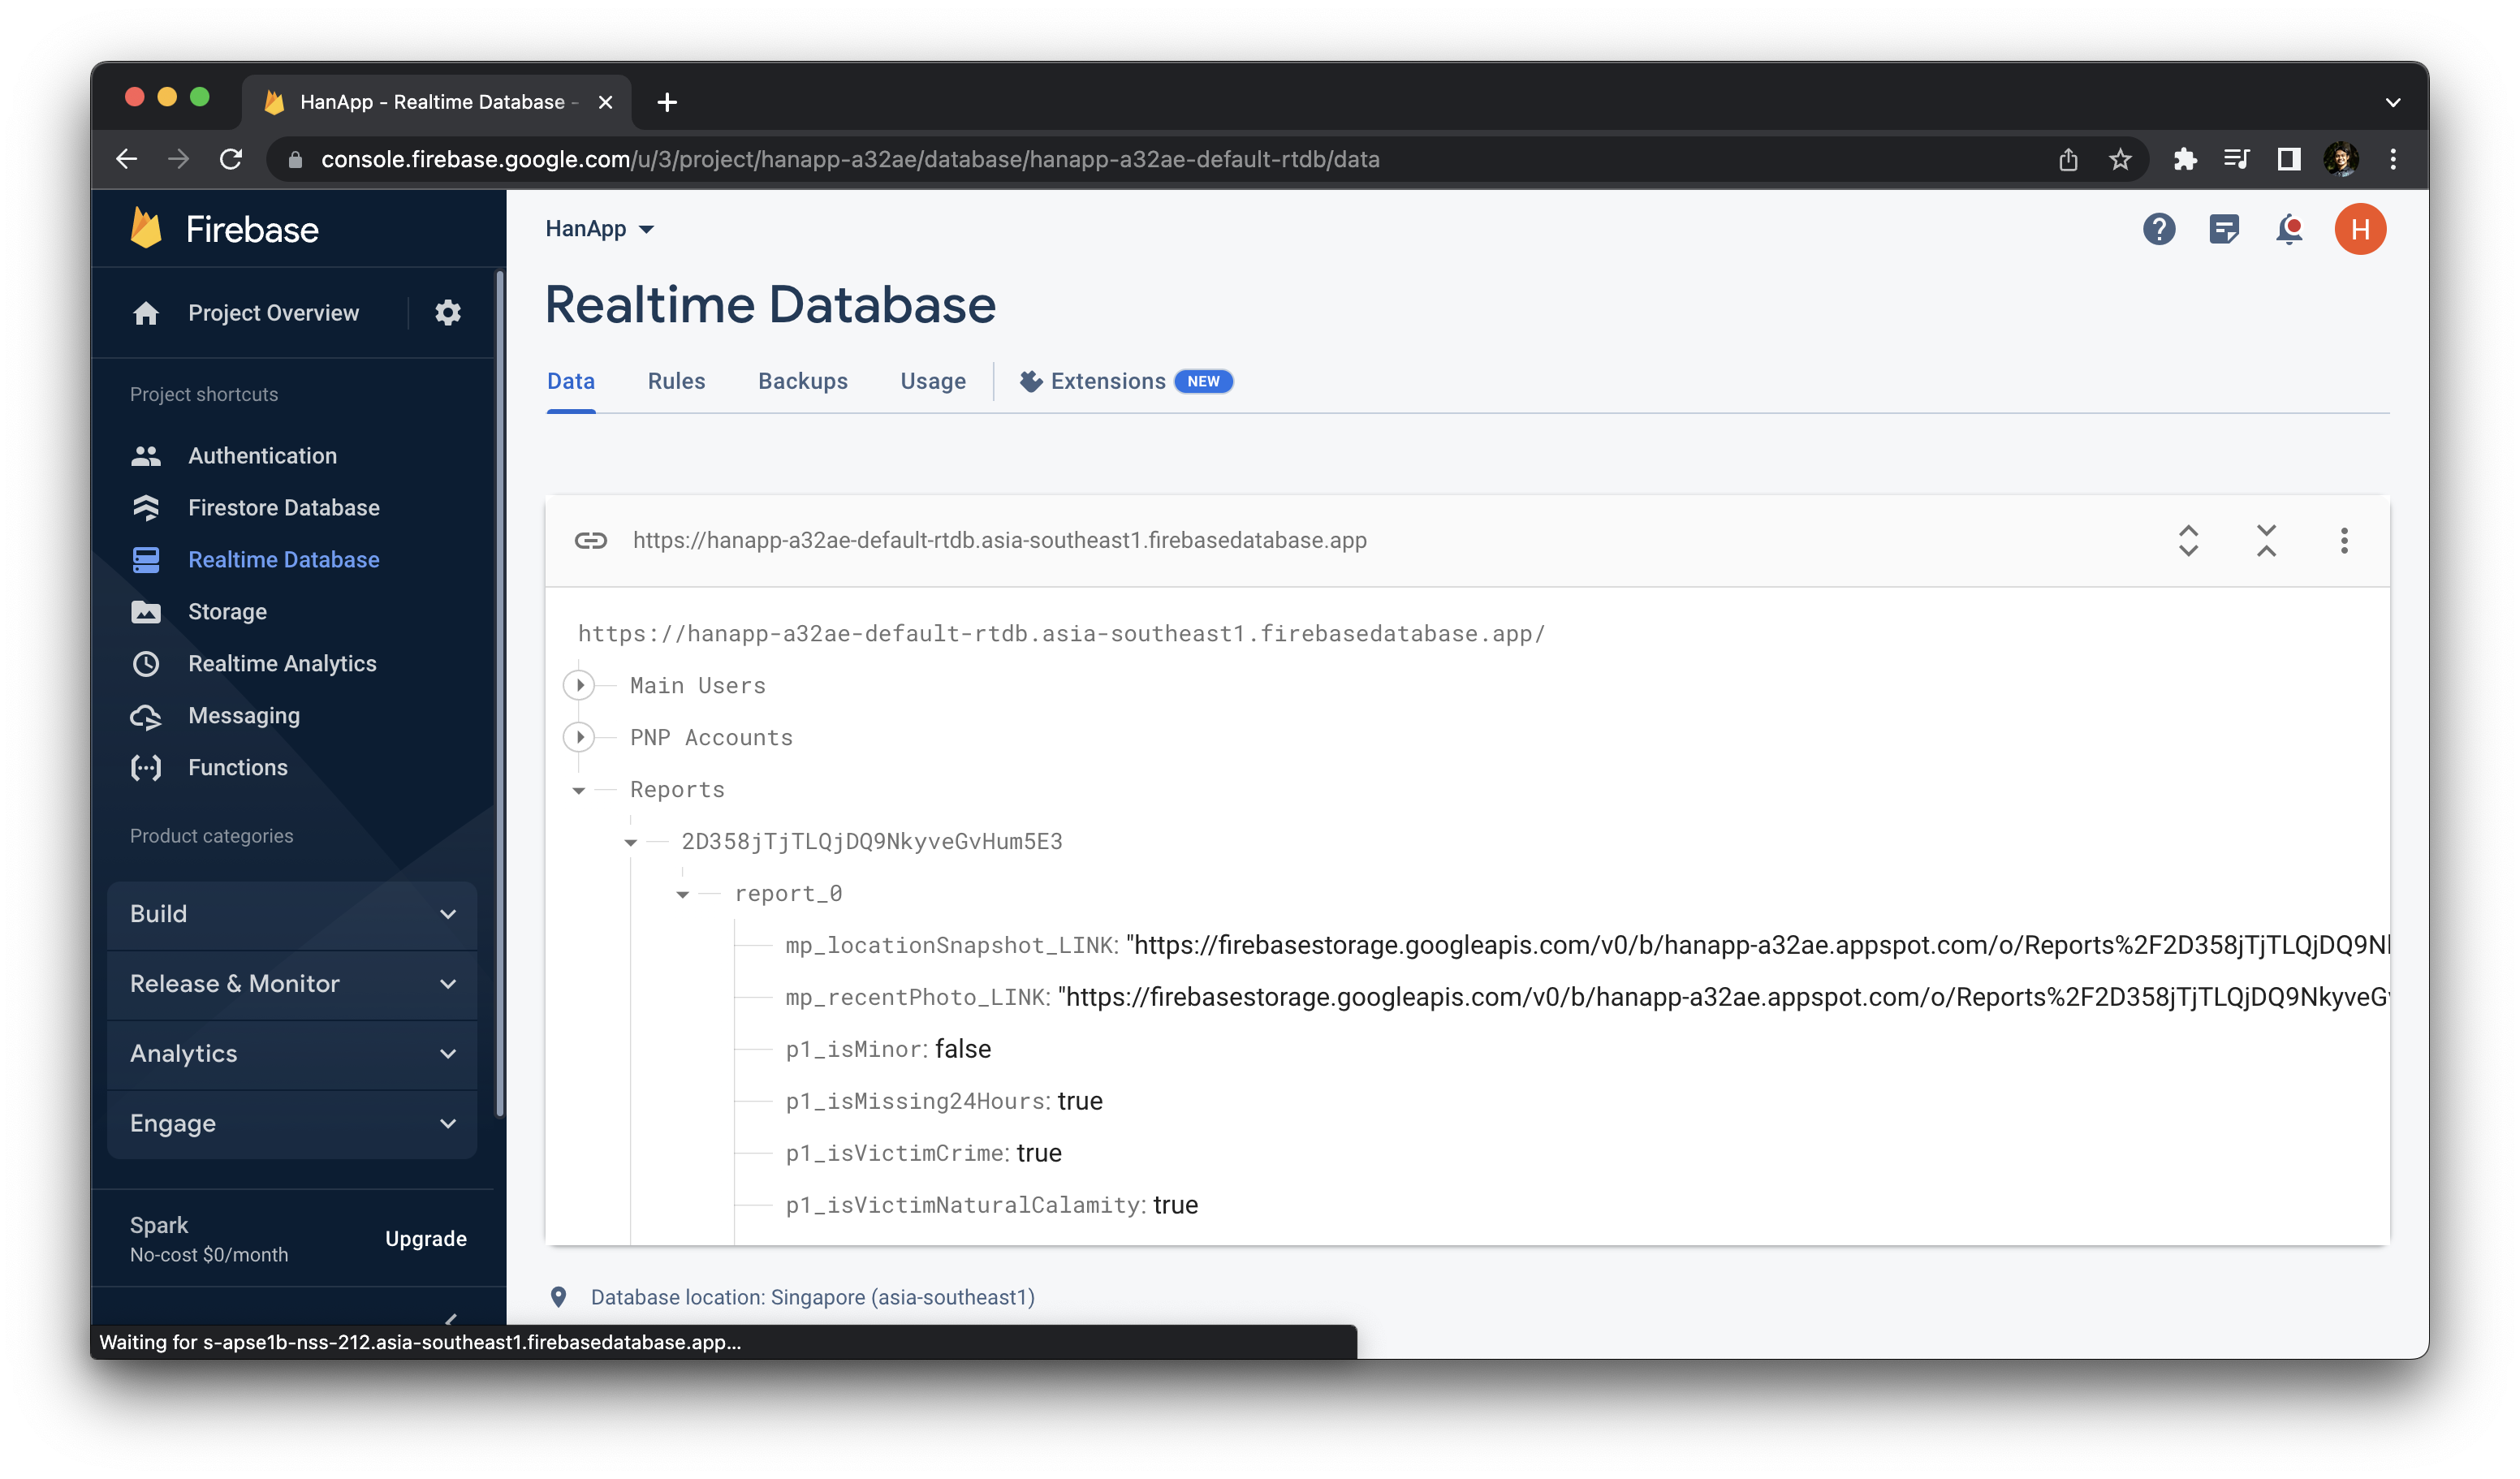
\includegraphics[scale=0.25]{figures/Chapter4/Firebase/rtdbReports.png}
        \caption{Realtime Database User Data and Reports}
        \label{fig:firebaseRTDB}
    \end{minipage}
\end{figure}
\subsubsection{Firebase Storage for Images Submitted in Reports}

Figure \ref{fig:firebaseStorage} contains all the images submitted in the reports including the reportee's signature. As seen in the header address line, images are organized under a "Reports" node, under each "User" node, and under each "Report Number" node. This setup allows for a more organized way of storing images submitted for easier retrieval.
\begin{figure}[!h]
    \centering
    \begin{minipage}[c]{1\linewidth}
        \centering
        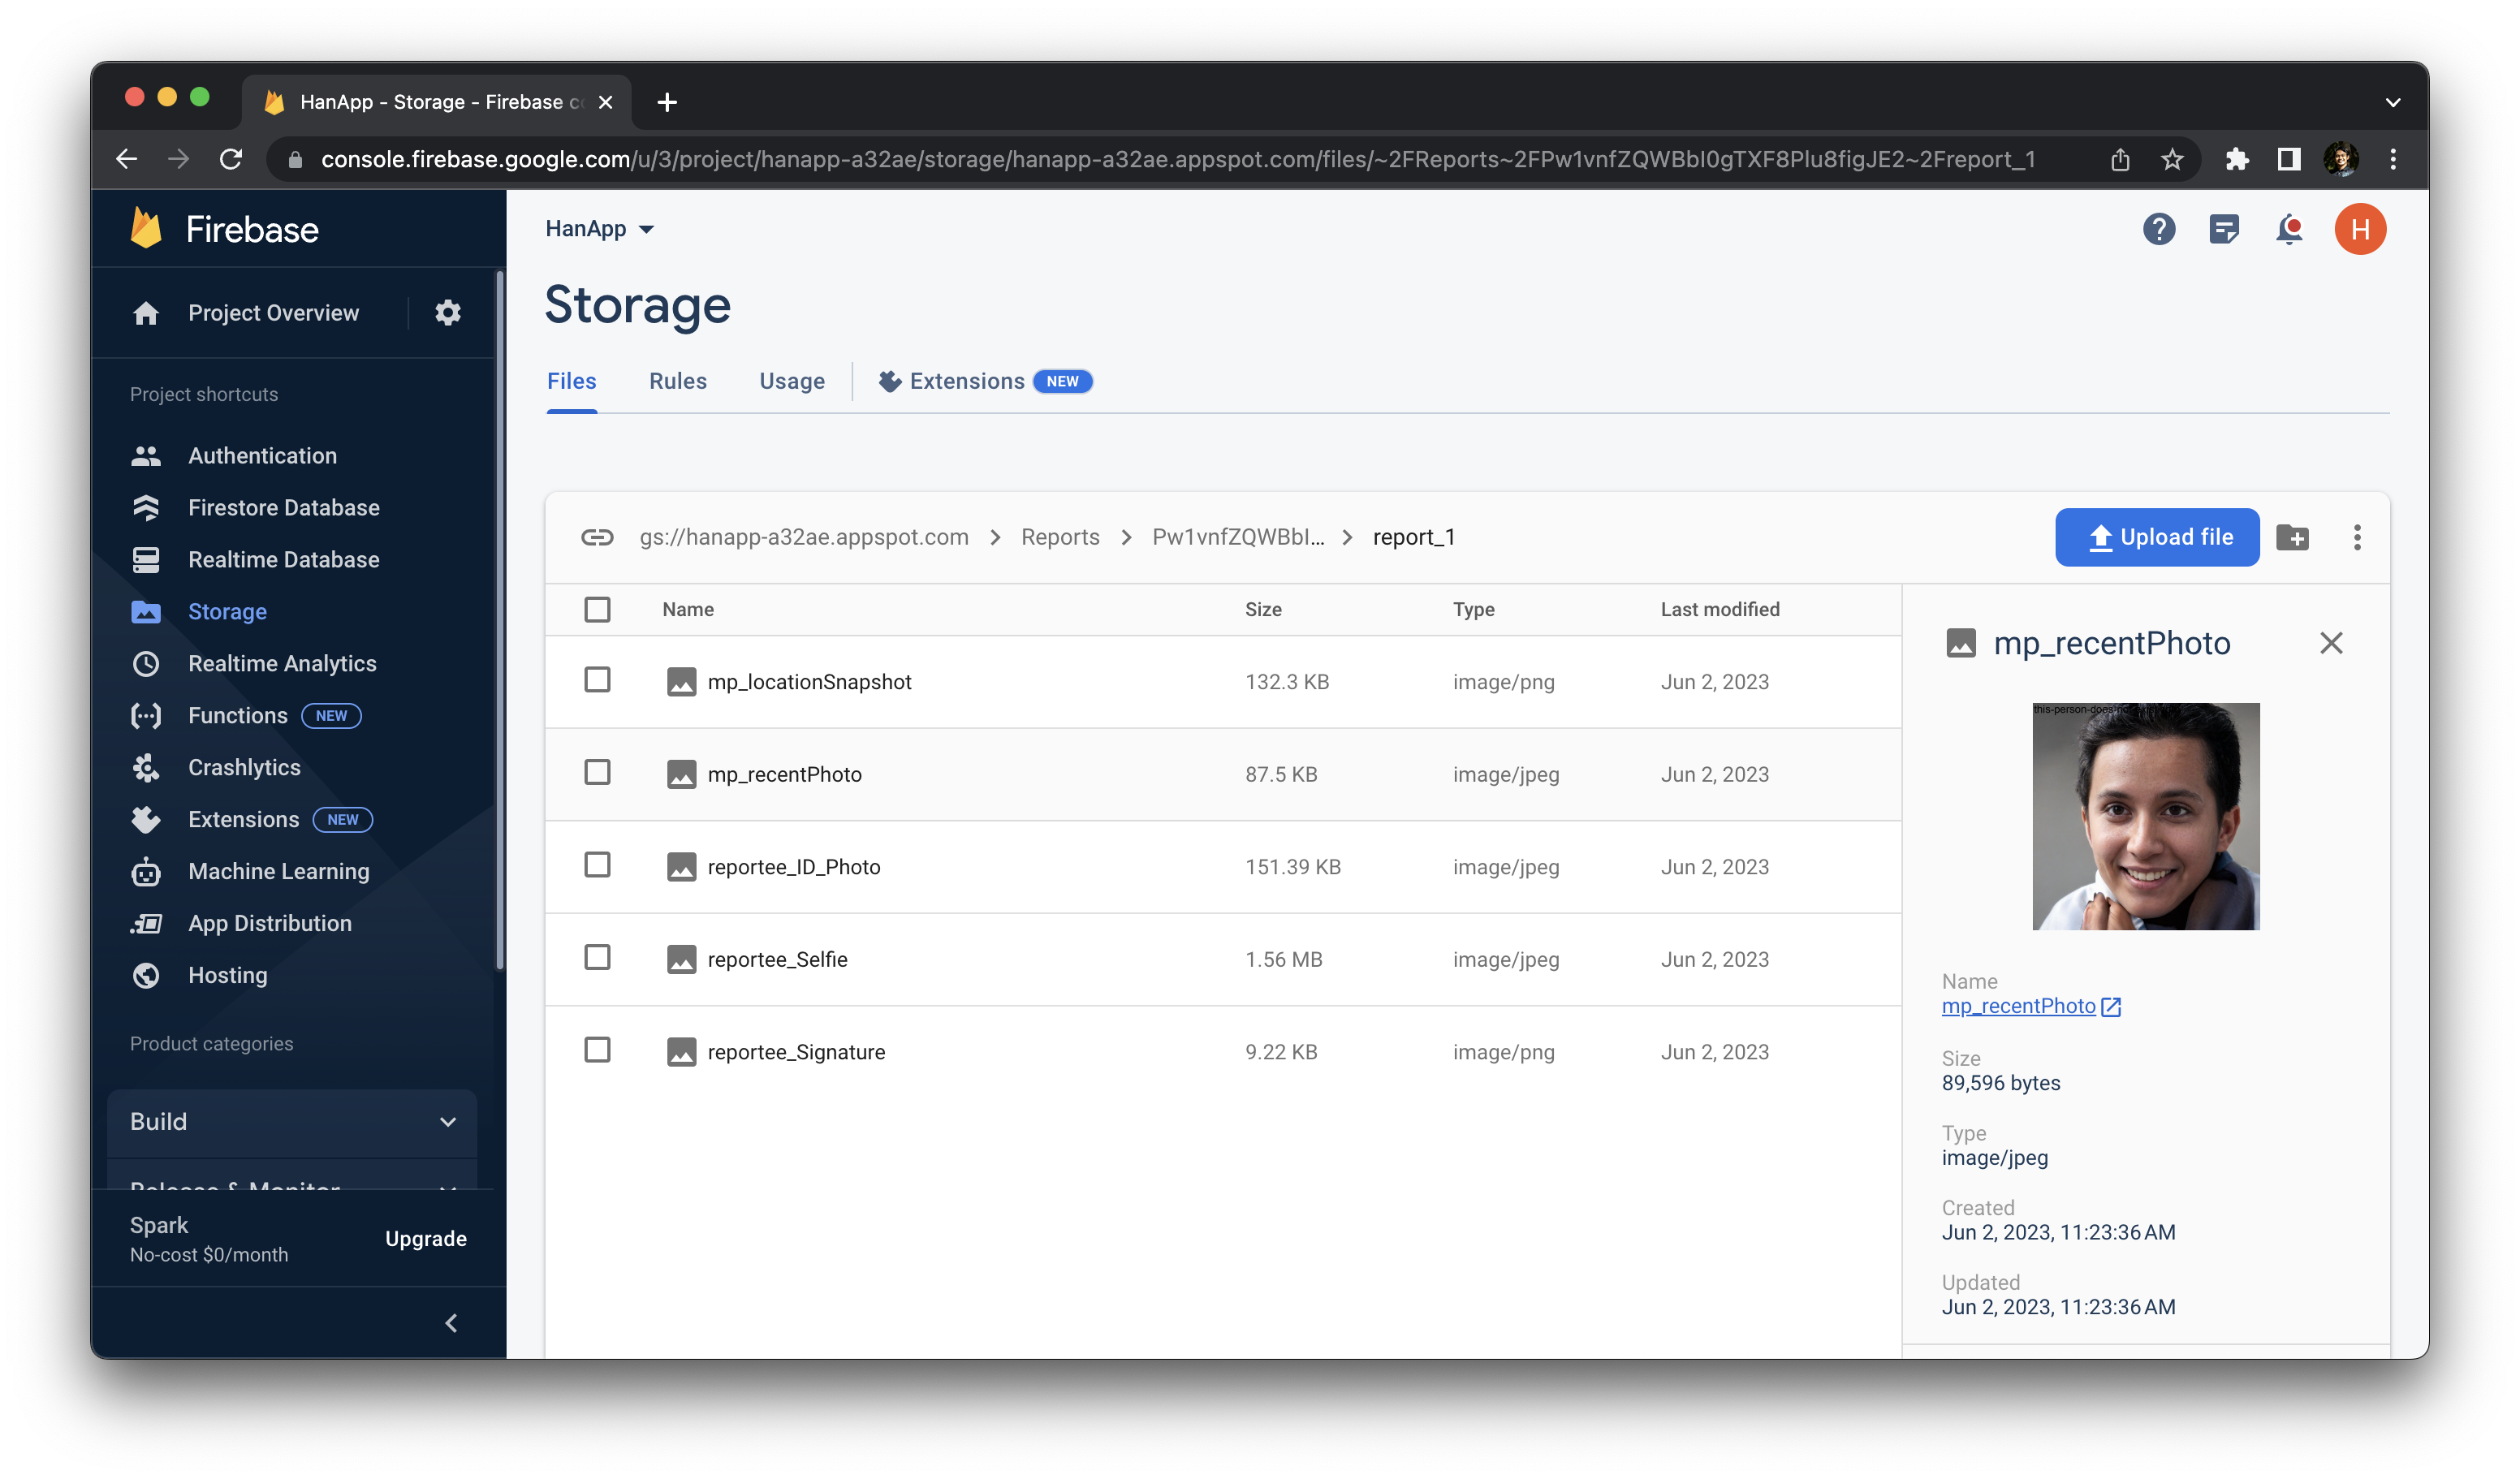
\includegraphics[scale=0.25]{figures/Chapter4/Firebase/storage.png}
        \caption{Firebase Storage}
        \label{fig:firebaseStorage}
    \end{minipage}
\end{figure}